\documentclass[../main.tex]{subfiles}

\begin{document}
\section{Problem Definition} \label{sec:definition}
Consider a homogeneous robotic team with $n$ robots in an indoor environment, with positions denoted as $x_i \in \mathbb{R}^2$ where $i \in \{1, 2, \ldots, n\}$, and single integrator dynamics of $\dot x_i = u_i$. Velocity limitation exists for the robots as $||u_i|| \leq u_{max}$. Each robot is able to communicate with all robots within a limited Euclidean distance $R$, which means that robot $i$ is connected and can communicate with robot $j$ if $||x_i - x_j|| \leq R$, with $i, j \in \{1, \ldots, n\}$. In this case, robot $j$ is considered as a neighbor of robot $i$. We denote the neighbor set of robot $i$ to be $\mathcal{N}_i$. This forms a spacially induced connectivity graph $\mathcal{G} = (\mathcal{V}, \mathcal{E})$ where each vertex $v_i \in \mathcal{V}$ represents robot $x_i$ in the environment, and each edge $e_{ij} \in \mathcal{E}$ between $v_i$ and $v_j$ exists when robot $i$ and robot $j$ is connected as defined above. With the definitions above, the connectivity graph $\mathcal{G}$ is undirected, i.e. $e_{ij} = e_{ji}$.

When the robots move, they maintain a safety distance with each other of $d_{ij} \geq r$ where $d_{ij} = ||x_i - x_j||$ and $r$ is the safety radius between the robot $i$ and $j$ to avoid collision. The robots also avoid obstacles in the environment by maintaining $||x_i - x_o|| \geq r$ where $x_o \in \mathcal{O}$ denotes the list of obstacles in the environment, which is known to the robots. To guarantee connectivity of the system as well as avoiding obstacles in the environment, we maintain the \textit{Minimum Connectivity Constraint Spanning Tree} \cite{luo2019behavior} with \textit{barrier certificate} \cite{borrmann2015control}.

Suppose some robots are assigned tasks and need to visit a sequence of locations in parallel, and the other robots are moving to keep the system connected, i.e. keep the connectivity graph $\mathcal{G}$ strongly connected. Consider a task mapping function specified as $s[i, t] = g_i$, where  $g_i \in \mathbb{R}^2$ denotes the goal location of robot $i$ at time $t$. We define those robots with assigned tasks to be \textit{task robots}. If robot $i$ does not have any assigned task at time $t$, i.e. $s[i, t] = \varnothing$, then robot $i$ is considered as a \textit{connection robot}, whose role is to maintain the connectivity of the robotic system and provide high flexibility for task robots to perform assigned tasks. We denote the set of connection robots to be $\mathcal{V}_c$ and the set of task robots to be $\mathcal{V}_t$. According to definition, we have $\mathcal{V}_c \cup \mathcal{V}_t = \mathcal{V}$. Since the robots are homogeneous, they can be either task robot or connection robot depending on task allocations and may switch roles accordingly.

\begin{figure}
    \centering
    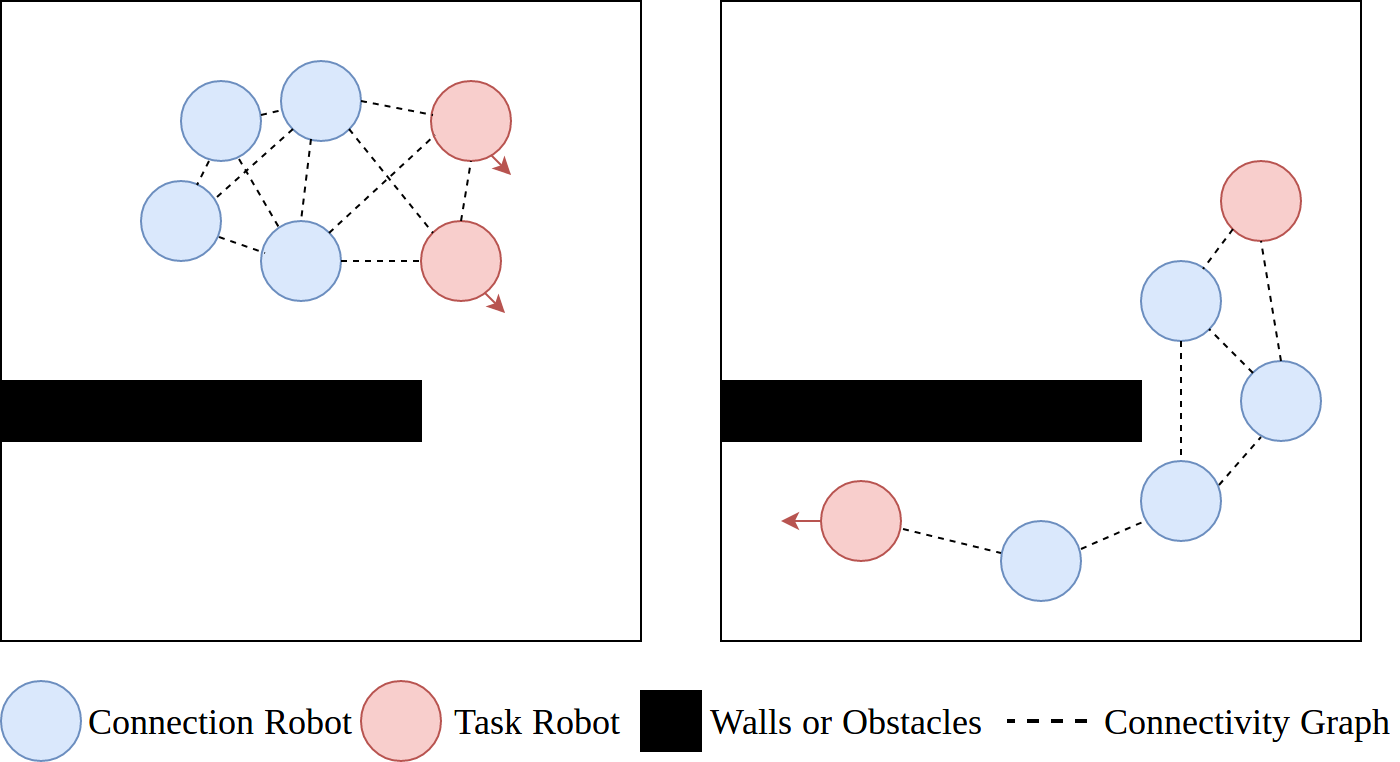
\includegraphics[width=0.8\textwidth]{topo_correct.png}
    \setlength{\belowcaptionskip}{-14pt}
    \caption{Two example scenarios for a system with robots allocated with tasks and connection robots. Left: connection robots need to keep up with task robots to avoid being left behind; Right: connection robots need to spread out so as to provide flexibility for the task robots to execute tasks.}
    \label{fig:prob_example}
\end{figure}

An illustrative example is shown in Figure~\ref{fig:prob_example} to demonstrate the possible functionality of the connection robots in an indoor environment. As shown in the figure, the red robots are the task robots and the blue robots are those without tasks and thus serving as connection robots to keep the system connected while others executing their tasks. The connection robots need to keep up with the task robots when the goal locations of the task robots are in a similar direction. In another example scenario when the goal locations of the task robots are far away from each other, the connection robots need to adjust the topology of the connectivity graph so as to provide maximum flexibility for the task robots to achieve their goal locations. The walls and task locations heavily influence the topology of the connectivity graph, thus having a huge impact on the overall performance.

As described in the example above, depending on the environment and task locations, the topology of the connectivity might change and could result in failing assigned tasks. In this case, it is essential for the connection robots to correct the unsuitable topology of the connectivity graph for better support of the task executions. Therefore, in this paper, our objective is to design a distributed controller for the connection robots to correct topology of the connectivity graph so as to maintain flexible connectivity of the robotic system.

\section{Topology Correction}
% In the previous section we introduced three types of constraints enforced on the robotics system: 1) collision avoidance with obstacles; 2) maintain connectivity within connectivity radius; and 3) avoiding collision between robots. Each of these is a hard constraint in the barrier certificate \cite{borrmann2015control}.

\subsection{Graph Laplacian and Convergence} \label{sec:laplacian}
Consider the \textit{graph Laplacian} matrix $L$ of the above mentioned connectivity graph $\mathcal{G}$. The graph Laplacian is defined as 
\begin{equation}\label{eq:laplacian} 
L = D - A
\end{equation}
where $A$ is the adjacency matrix where each element $a_{ij}=1$ if an edge exists between $v_i$ and $v_j$, and zero otherwise. $D = \text{diag}(deg(1), \ldots, deg(n))$ is the degree matrix where each $deg(i)$ denotes the degree of vertex $v_i$ that $deg(i) = \sum_{i \neq j} a_{ij}$, and zero off-diagonal elements. By definition, $L$ is symmetric if the graph is undirected, and has a right eigen vector of $\mathbf{1}$ and zero eigenvalue, i.e. $L \cdot \mathbf{1} = 0 \cdot \mathbf{1}$.

Laplacian matrix $L$ of the connectivity graph is essential for evaluating the convergence of consensus algorithms. The eigenvalues of $L$ can be computed and sorted in ascending order, denoted as
\begin{equation} 
    \lambda_1(L) \leq \lambda_2(L) \leq \ldots \leq \lambda_n(L)
\end{equation}
The smallest eigenvalue $\lambda_1(L)$ of the Laplacian matrix is always zero as mentioned above. The second smallest eigenvalue $\lambda_2(L)$ describes the \textit{algebraic connectivity} of the graph \cite{fiedler1973algebraic}. Let $\delta = \min deg(i)$ to be the minimum degree of the vertices in graph $\mathcal{G}$ with $n$ vertices. A lower bound for the algebraic connectivity $\lambda_2(L)$ exists \cite{de2007old}
\begin{equation}\label{eq:lambda_bound} 
\lambda_2(L) \geq 2 \delta - n + 2
\end{equation}
It is known that a continuous-time consensus is globally exponentially reached with a speed that is faster or equal to $\lambda_2(L_s)$ where $L_s = (L + L^T)/2$ for a strongly connected balanced digraph \cite{olfati2007consensus}. For undirected graph with a symmetric Laplacian matrix, we have $L = L_s = (L + L^T)/2$. In our setting, the speed of convergence is $\lambda_2(L)$. 

Therefore, to achieve a faster convergence rate, the controller of the connection robots aims at correcting the topology of connectivity graph by  \textit{maximizing the minimum degree $\delta$}.

\subsection{Weighted Rendezvous}
To keep the robotics system connected, it is straight forward to execute \textit{rendezvous} on the connection robots so that they could keep up with the task robots. A common control law used for rendezvous \cite{olfati2007consensus} is
\begin{equation} 
\dot x_i(t) = \sum_{j \in \mathcal{N}_i} a_{ij}(x_j(t) - x_i(t))
\end{equation}
where $\mathcal{N}_i$ denotes the neighbor set of robot $i$ as introduced in section \ref{sec:definition} and $a_{ij}$ is the element in adjacency matrix. However, this pure rendezvous controller will result in clusters of robots, making it hard for the non-connection robots to execute tasks. Following the discussion in section \ref{sec:laplacian}, we propose the \textit{weighted rendezvous} as follows
\begin{equation}\label{eq:weighted_rend} 
\dot x_i(t) = \sum_{j \in \mathcal{N}_i} w_{ij}^r(x_j(t) - x_i(t))
\end{equation}
where the weight $w_{ij}^r$ in the weight array $\mathbf{w}_i^r = \left[w_{i1}^r, \ldots, w_{ij}^r, \ldots, w_{i|\mathcal{N}_i|}^r\right]$, where $j \in \mathcal{N}_i$.

\subsubsection{Degree-based Weighted Rendezvous} \label{sec:degree_rend}
Following the discussion in section \ref{sec:laplacian}, we may set the weights with respect to the degree of neighboring vertices. The weights should be larger on vertices with smaller degrees and smaller on vertices with larger degrees. Therefore, the desired weights are calculated as 
\begin{equation}  \label{eq:degree_weight}
\mathbf{w}_i^r = \max deg(\mathcal{N}_i) - deg(\mathcal{N}_i) + \epsilon
\end{equation}
where $deg(\mathcal{N}_i)$ denotes the degree array of the neighboring vertices where each element is the degree of a neighbor vertex $deg(j)$, $j \in \mathcal{N}_i$ and $|deg(\mathcal{N}_i)| = |\mathcal{N}_i|$. The variable $\epsilon$ is a small value of $1 \gg \epsilon > 0$ and serves as a \textit{correction factor} to guarantee that weights are not all zeros with complete graph (the graph that every pair of vertices is connected). The weight array is then normalized so that $\sum_{j \in \mathcal{N}_i}w_{ij}^r = 1$.

We will then prove that this controller will correct the topology of connectivity graph by modifying the minimum degree $\delta$ of graph $\mathcal{G}$.
\begin{figure}
    \centering
    \includegraphics[width=0.36\textwidth]{graph_vertex.png}
    \setlength{\belowcaptionskip}{-14pt}
    \caption{The moment when vertex $v_j$ is moving to $v_k$ resulting in $v_i$ and $v_j$ getting disconnected from each other.}
    \label{fig:graph_vertex}
\end{figure}

An assumption made in this paper is that time discretization is dense enough so that only one edge will change (connect or disconnect) at each time step. Before we start the proof, we list several cases of topology changes that we are not interested in:
\begin{itemize}
\item Adding an edge: when two robots come closer and new connection is made, it can only cause an increase of minimum degree $\delta$.
\item Removing an edge $e_{ij}$ where $deg(i) > \delta$ and $deg(j) > \delta$: when two robots $i$ and $j$ move away from each other with a distance larger than $R$, the connection edge $e_{ij}$ is removed. Let $deg(i, t)$ denotes the degree of vertex $v_i$ at time $t$. When originally at time $t$, $deg(i, t) > \delta$, notice that degrees are integers, we have $deg(i, t) \geq \delta + 1$. Thus, if $e_{ij}$ is removed in the next time step, we still have $deg(i, t+1) \geq \delta$, similar inequality holds for $v_j$. The minimum degree $\delta$ is not influenced in the case.
\end{itemize}
Therefore, the only case that is of our interest is shown in Figure~\ref{fig:graph_vertex}, which describes the case when the vertex $v_i$ having minimum degree $deg(i, t) = \delta$, and $v_j$ is moving towards its other neighbor $v_k$, causing edge $e_{ij}$ to disconnect. This is the only case that will cause a decrease of $\delta$ and in the following proof of theorem~\ref{thm:delta_increase}, the following discussion focuses on this case.

\begin{preposition} \label{thm:delta_increase}
With the control law defined in equation~\ref{eq:weighted_rend} with weights defined in equation~\ref{eq:degree_weight}, the minimum degree $\delta$ of connectivity graph increases, i.e. $\delta(t+1) \geq \delta(t)$, where $\delta(t)$ denotes the minimum degree at time $t$. 
\end{preposition}
\begin{proof}
We prove by contradiction.

As described above, the only case that will result in $\delta(t) > \delta(t+1)$ is shown in Figure~\ref{fig:graph_vertex} when vertex $v_j$ moves towards $v_k$ and disconnects with vertex $v_i$ where $deg(i, t) = \delta(t)$ at time $t$. According to equation~\ref{eq:weighted_rend}, $\dot x_j(t)$ moves towards $x_k(t)$ results from $w_{jk}^r > w_{ji}^r$. Then we have
{\small \begin{align*}
w_{jk}^r &= \max deg(\mathcal{N}_j) - deg(k) + \epsilon \\
&> \max deg(\mathcal{N}_j) - deg(i) + \epsilon = w_{ji}^r
\end{align*}}
Thus we have
\begin{equation} 
    deg(i) = \delta(t) > deg(k)
\end{equation}
This violates the initial assumption that $v_i$ with $deg(i, t) = \delta(t)$ at time $t$ has the minimum degree. Therefore, the case described above will not happen and any other scenarios will not result in decrease of $\delta$, thus $\delta(t+1) \geq \delta(t)$.
\end{proof}

\subsubsection{Distance-based Weighted Rendezvous}
The degree-based approach introduced in the previous section is able to trigger edge changes so as to increase the convergence rate by gradually modifying the minimum degree $\delta$ in the graph. We notice that this degree-based approach treats all graphs with the same vertex and edge set the same, without considering the actual physical distance between vertices. To further optimize our objective, we propose the \textit{distance-based weighted rendezvous} based on the degree-based approach that provides the same guarantees and better performance.

We first define a \textit{density score} of each vertex $v_i$ as
\begin{equation}  \label{eq:density_score}
c(i) = deg(i) + \sum_{j \in \mathcal{N}_i} \frac{R - d_{ij}}{deg(i) (R - r)} 
\end{equation}
The density score $c(i)$ describes the level of density around vertex $v_i$. An intuition on this is that when the neighboring robots are close to robot $i$, $d_{ij}$ is relatively small, then density score of robot $i$ is higher, and vice versa. Similarly, the weights are calculated as
\begin{equation}  \label{eq:distance_weight}
\mathbf{w}^r_i = \max c(\mathcal{N}_i) - c(\mathcal{N}_i) + \epsilon
\end{equation}
where $1 \gg \epsilon >0$ is the same \textit{correction factor} as in previous section. The weight array is then normalized such that $\sum_{j \in \mathcal{N}_i}w_{ij}^r = 1$ for each robot $i$. We will then prove that this formulation gives the same guarantee as equation~\ref{eq:degree_weight}.

\begin{lemma}\label{lm:c_deg_relation}
For any two connected vertices $v_i, v_j \in \mathcal{V}$, $e_{ij} \in \mathcal{E}$ on graph $\mathcal{G} = (\mathcal{V}, \mathcal{E})$, if $deg(i) > deg(j)$, then $c(i) \geq c(j)$.
\end{lemma}
\begin{proof}
We prove by analyzing the relationship of $deg(i)$ and $c(i)$ for vertex $v_i$.

Since $d_{ij} = ||x_i - x_j||$ when $e_{ij} \in \mathcal{E}$, we have
\begin{equation} \label{eq:d_r_R}  
r \leq d_{ij} \leq R
\end{equation}
where as defined in section~\ref{sec:definition} that $r$ is the safety radius and $R$ is the connectivity radius. By applying the inequality in equation~\ref{eq:d_r_R}, we have
{\small \begin{align*}
c(i) &= deg(i) + \sum_{j \in \mathcal{N}_i} \frac{R - d_{ij}}{deg(i) (R - r)} \\
&\geq deg(i) + \sum_{j \in \mathcal{N}_i} \frac{R - R}{deg(i) (R - r)} = deg(i)
\end{align*}}
Notice that $deg(i) = |\mathcal{N}_i|$, we also have
{\small \begin{align*}
c(i) &= deg(i) + \sum_{j \in \mathcal{N}_i} \frac{R - d_{ij}}{deg(i) (R - r)} \\
&\leq deg(i) + \sum_{j \in \mathcal{N}_i} \frac{R - r}{deg(i) (R - r)} = deg(i) + 1
\end{align*}}
Combining the two equations above we get
\begin{equation} 
deg(i) \leq c(i) \leq deg(i) + 1
\end{equation}
Notice that degree of vertex is integer. The inequality $deg(i) > deg(j)$ is the same as $deg(i) \geq deg(j) + 1$. Therefore we have
\begin{equation} 
c(i) \geq deg(i) \geq deg(j) + 1 \geq c(j)
\end{equation}
Then we may conclude that $c(i) \geq c(j)$ holds when $deg(i) > deg(j)$.
\end{proof}
We are then able to show our final statement. It is proven in Lemma~\ref{lm:c_deg_relation} that density score preserves the inequality of the degree values. Following the same procedure of the proof for Prepostion~\ref{thm:delta_increase}, we may conclude that $\delta$ increases similarly for the density score defined in equation~\ref{eq:density_score}. Therefore, the following theorem holds.
\begin{theorem}
With the control law defined in equation~\ref{eq:weighted_rend} with weights defined in equation~\ref{eq:distance_weight}, the minimum degree $\delta$ of connectivity graph increases, i.e. $\delta(t+1) \geq \delta(t)$, where $\delta(t)$ denotes the minimum degree at time $t$. 
\end{theorem}

With this distance-based weighted rendezvous, the connection robots will be able to keep up with the task robots and provide a flexible topology for the whole system.

\subsection{Weighted Flocking}
While weight rendezvous may solve the problem when task robots are moving away from the cluster of connection robots, weighted flocking introduced in this section may solve the problems caused by the scenario when task robots are moving through a cluster of connection robots. When there are many connection robots within the system, it is possible that they block the way of the task robots. An example of this is shown in Figure~\ref{fig:flock_block} when the task robot tries to move through a cluster of connection robots.
\begin{figure}
    \centering
    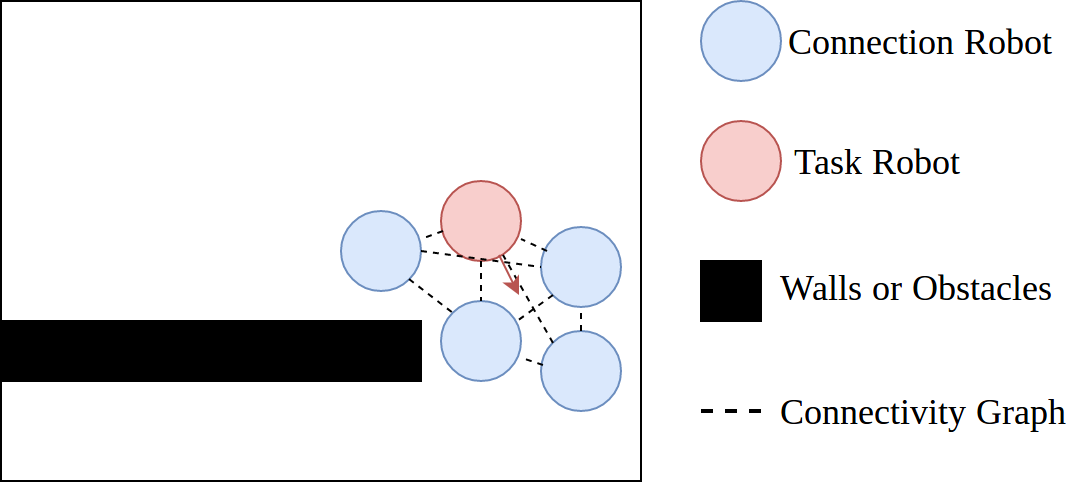
\includegraphics[width=0.6\textwidth]{flock_block.png}
    \caption{An example when the task robot is trying to move to an assigned location but the connection robots are cluttered along the way.}
    \label{fig:flock_block}
\end{figure}

To solve the problem mentioned above, we propose \textit{weighted flocking} as follows
\begin{equation} 
\dot x_i = \sum_{j \in \mathcal{N}_i} w_{ij}^f u_j
\end{equation}
The weights are designed so that the connection robots flocks with the neighboring task robots. 
\begin{equation} 
w_{ij}^f = 
\begin{cases}
\frac{1}{|\mathcal{V}_t \cap \mathcal{N}_i|}, & \text{if $v_j \in \mathcal{V}_t$}\\
0, &\text{otherwise}
\end{cases}
\end{equation}
where $|\mathcal{V}_t \cap \mathcal{N}_i|$ is the number of task robots in the neighbors of robot $i$.

\subsection{Weighted Behavior Combination}
The final resulting controller of the connection robots is designed as a \textit{weighted behavior combination} that combines the output from both weighted rendezvous and weighted flocking.

Denote the output velocity with weighted rendezvous as $u^r_i$ and the output velocity with weighted flocking as $u^f_i$ for robot $i$. We then calculate the weights of performing weighted flocking for each robot
\begin{equation} 
\alpha_i = \frac{1}{2u_{max}}\left|\left|u_i^r - \frac{1}{|\mathcal{V}_t \cap \mathcal{N}_i|} \sum_{j \in \mathcal{V}_t \cap \mathcal{N}_i}u_j\right|\right| \cdot \gamma
\end{equation}
where $\gamma \in (0, 1]$ is an environment-dependent value that controls the range of $\alpha_i$ since $\alpha_i \in (0, \gamma]$. $\gamma$ should be smaller with a very cluttered environment, and could be larger in an environment with relative sparse obstacles.

The controller of weighted behavior mixing for connection robots is then designed as
\begin{equation} 
\dot x_i = (1 - \alpha_i) u_i^r + \alpha_i u_i^f
\end{equation}
This method is also fully decentralized. Note that for weighted rendezvous and weighted flocking, each connection robot only needs to know the neighbor states to calculate the degree and density score, and then report to its neighbors. This distributed consensus-based method is very scalable with an increasing number of robots in the system, which we will show in the next section.

\section{Results}
\begin{figure}
\centering
\begin{subfigure}{0.28\textwidth}

\includegraphics[width=\textwidth]{map_3.jpg}
 
\caption{}
\label{fig:map_1}
\end{subfigure}
\begin{subfigure}{0.28\textwidth}
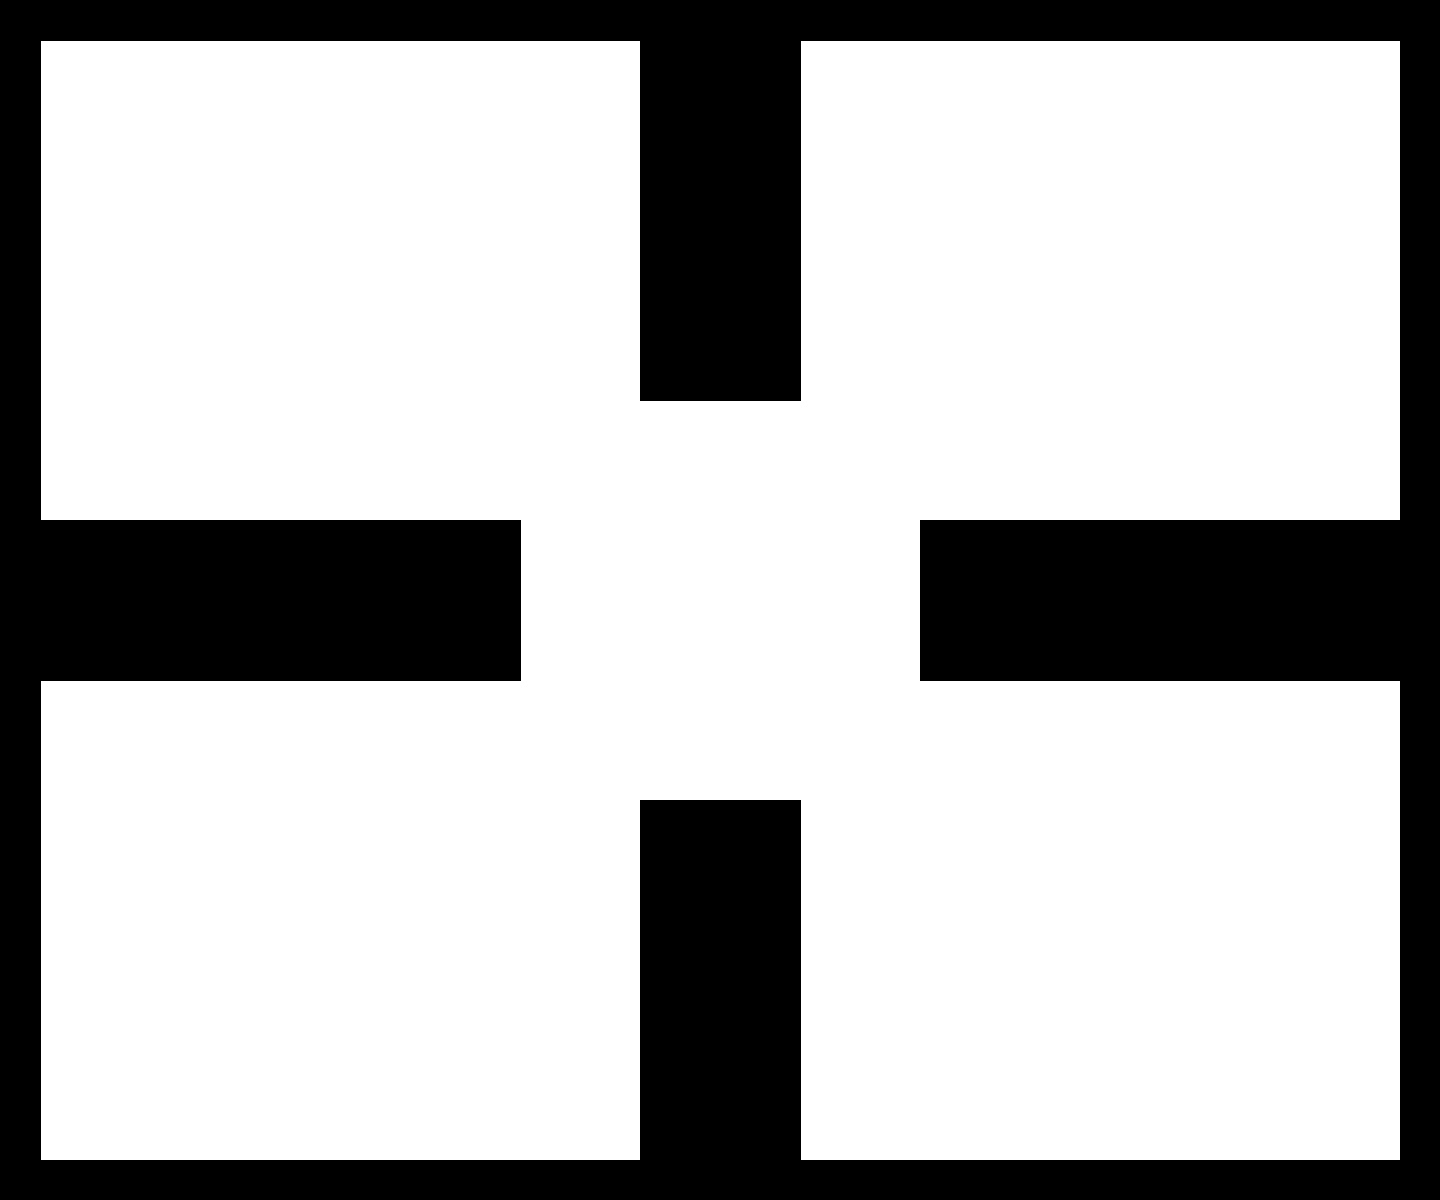
\includegraphics[width=\textwidth]{map_4.jpg}
 
\caption{}
\label{fig:map_2}
\end{subfigure}
\begin{subfigure}{0.34\textwidth}
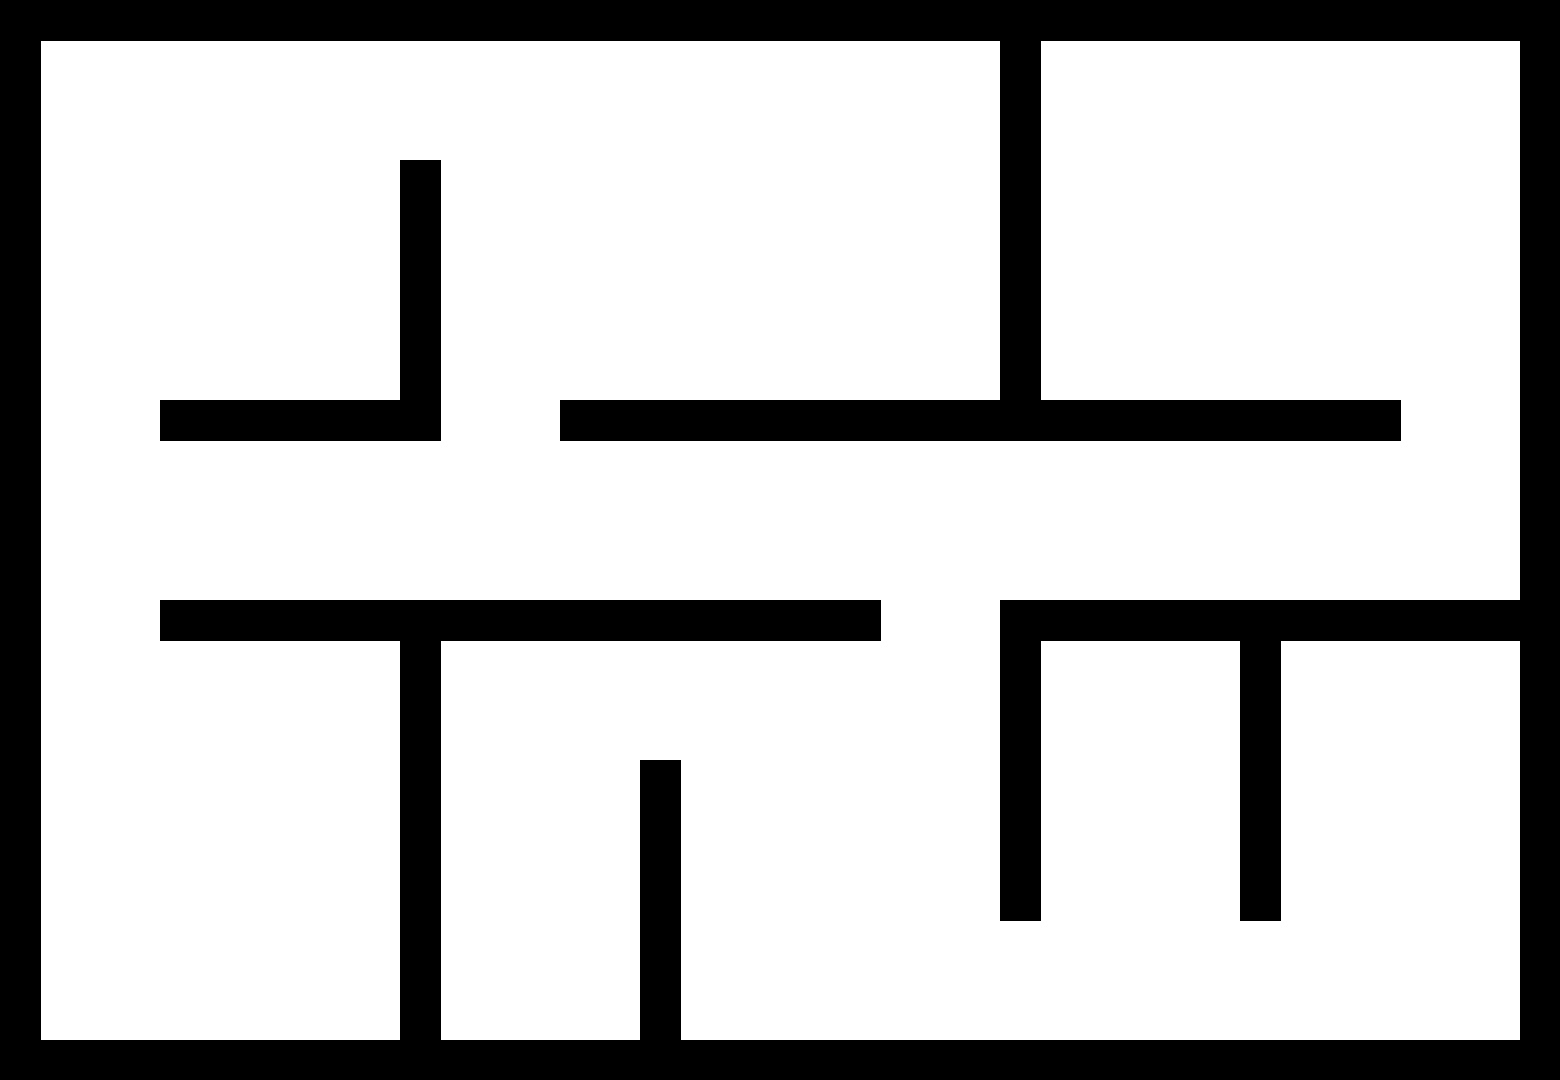
\includegraphics[width=\textwidth]{map_0.jpg}
 
\caption{}
\label{fig:map_3}
\end{subfigure}
\caption{(a) size 30$\times$36, (b) size 30$\times$36, and (c) size 27$\times$39, are the three maps for the experiments. The black area is the walls or obstacles in the environment, and the white area is the free space.}
\label{fig:maps}
\end{figure}
We tested our controller with the maps in Figure~\ref{fig:maps}. In map  \ref{fig:map_1}, the task robots have a sequence of similar goal locations. The challenge for the connection robots in this setting is to avoid blocking the way for the task robots. In map \ref{fig:map_2}, the goal locations for the task robots are relatively far from each other in each step. The challenge here is that the connection robots need to stretch out so as to keep the task robots far away connected.

\begin{figure}
\centering
% \vspace*{-0cm}
\begin{subfigure}{0.49\textwidth}
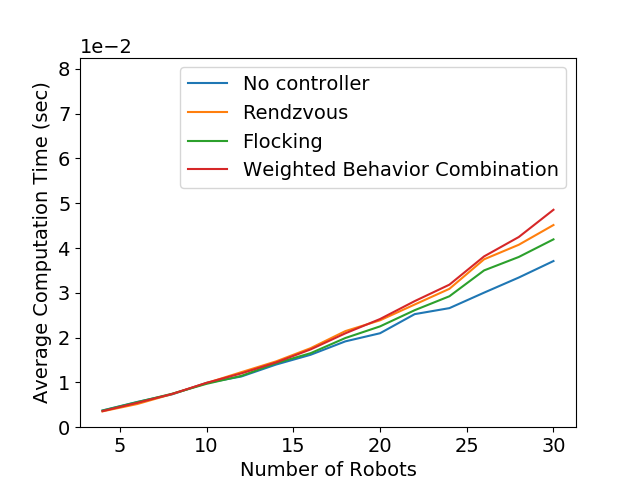
\includegraphics[width=\textwidth]{img/new_avg_time.png}
\caption{}
\label{fig:avg_time}
\end{subfigure}
\begin{subfigure}{0.49\textwidth}
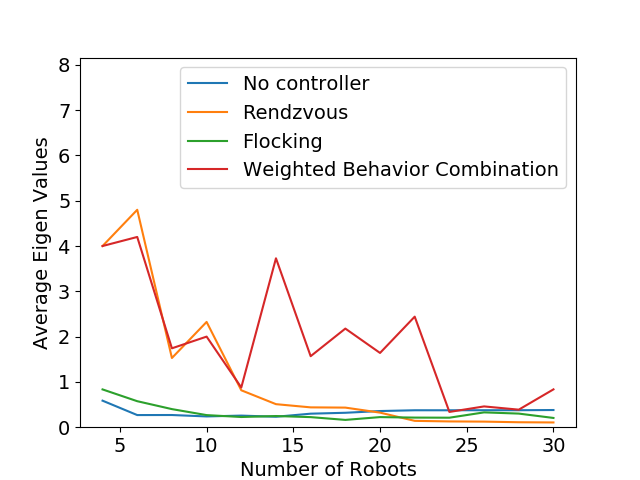
\includegraphics[width=\textwidth]{img/new_eigen.png}
\caption{}
\label{fig:eigen}
\end{subfigure}
\begin{subfigure}{0.49\textwidth}
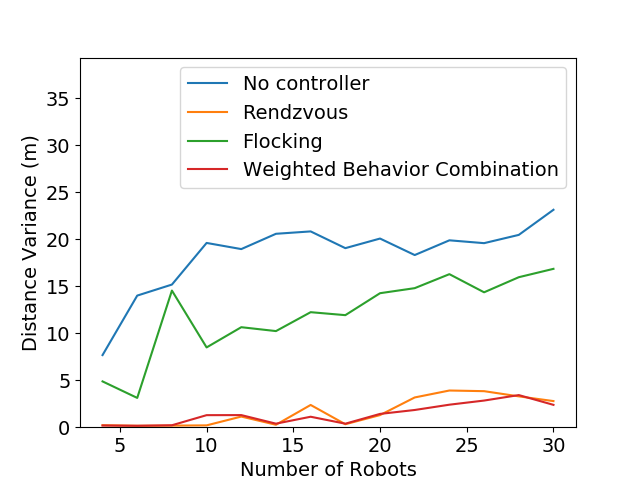
\includegraphics[width=\textwidth]{img/new_dis_var.png}
\caption{}
\label{fig:dis_var}
\end{subfigure}
\begin{subfigure}{0.49\textwidth}
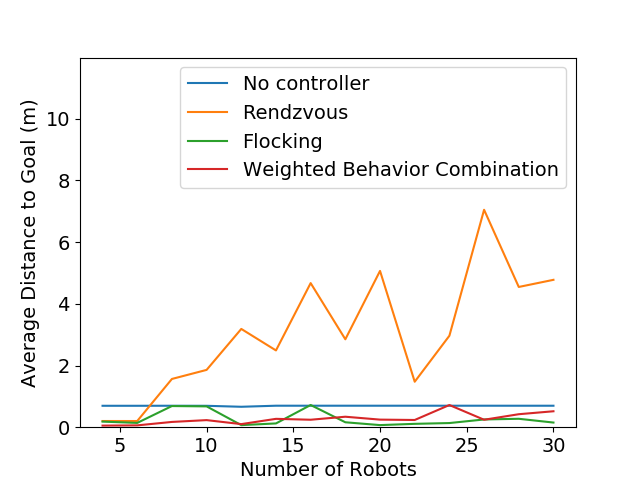
\includegraphics[width=\textwidth]{img/new_avg_dis.png}
\caption{}
\label{fig:avg_goal}
\end{subfigure}
\caption{(a) Average computation time for each iteration; (b) Average eigenvalues (c) Variance of the robot locations at each time of convergence; (d) Average distance to goal for the task robots at each time of convergence}
\label{fig:dis_goal}
\end{figure}

\begin{figure}
\centering
\begin{subfigure}[b]{0.24\textwidth}
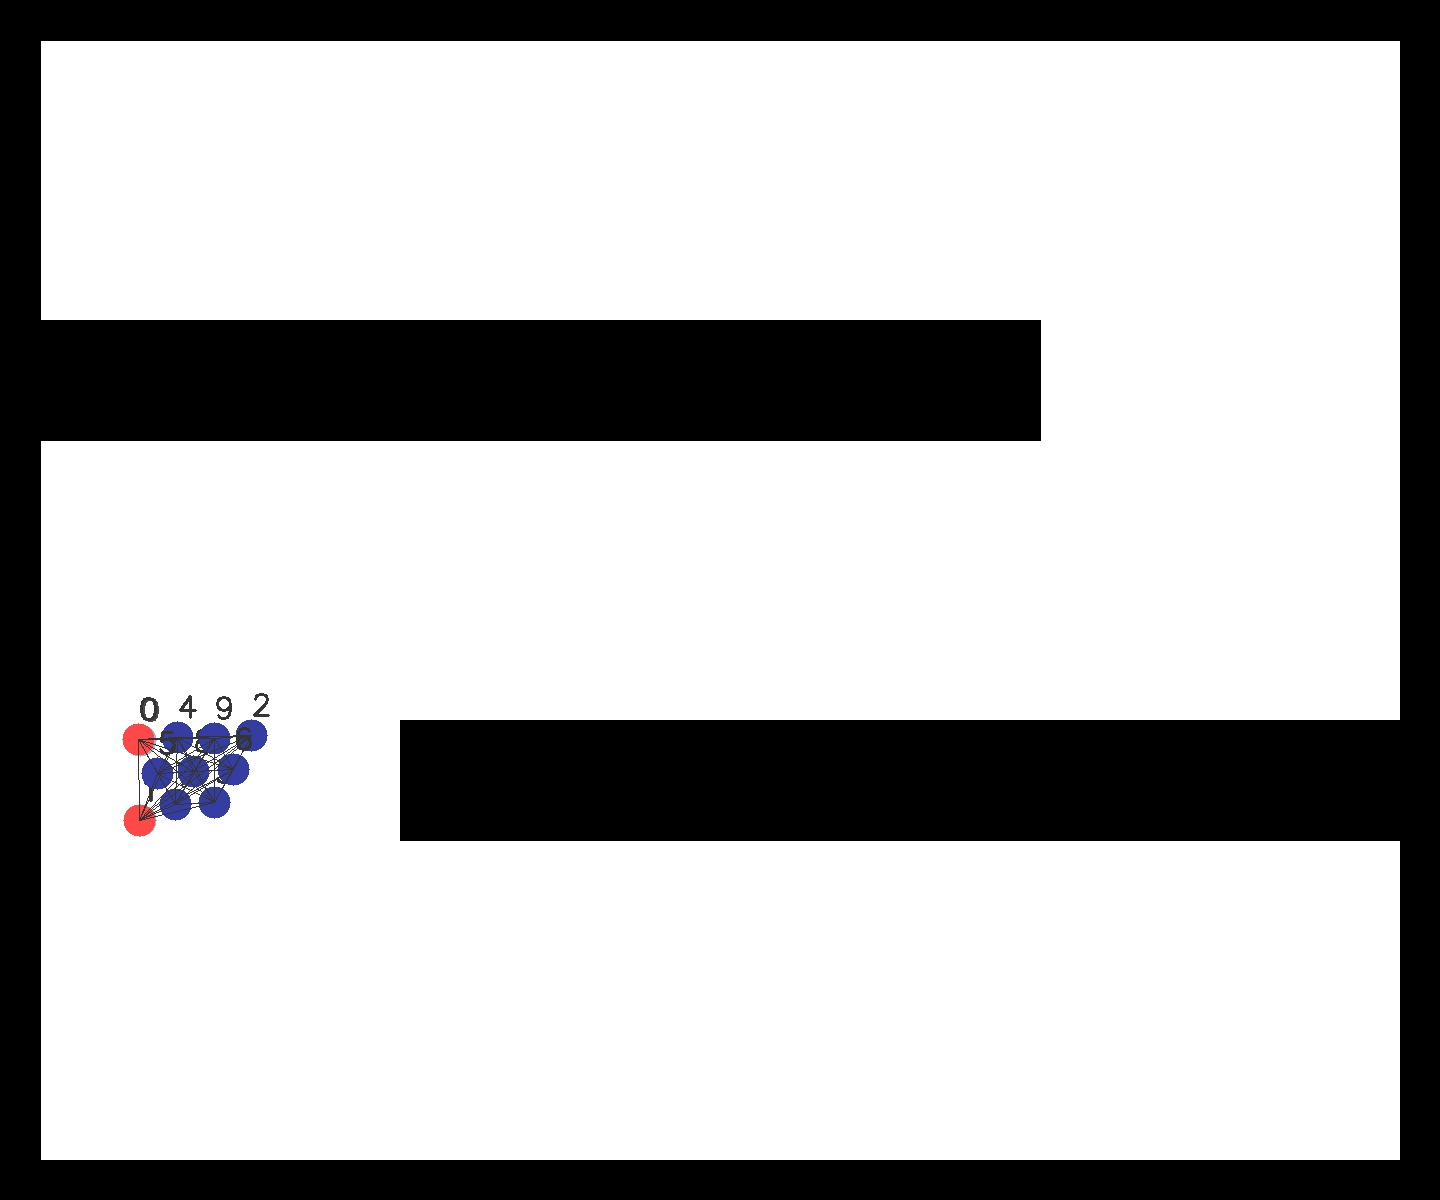
\includegraphics[width=\textwidth]{m3_mt3_1.jpg}
\caption{Task 2 Weighted Behavior Combination}
\label{fig:m3_mt3_1}
\end{subfigure}
\begin{subfigure}[b]{0.24\textwidth}
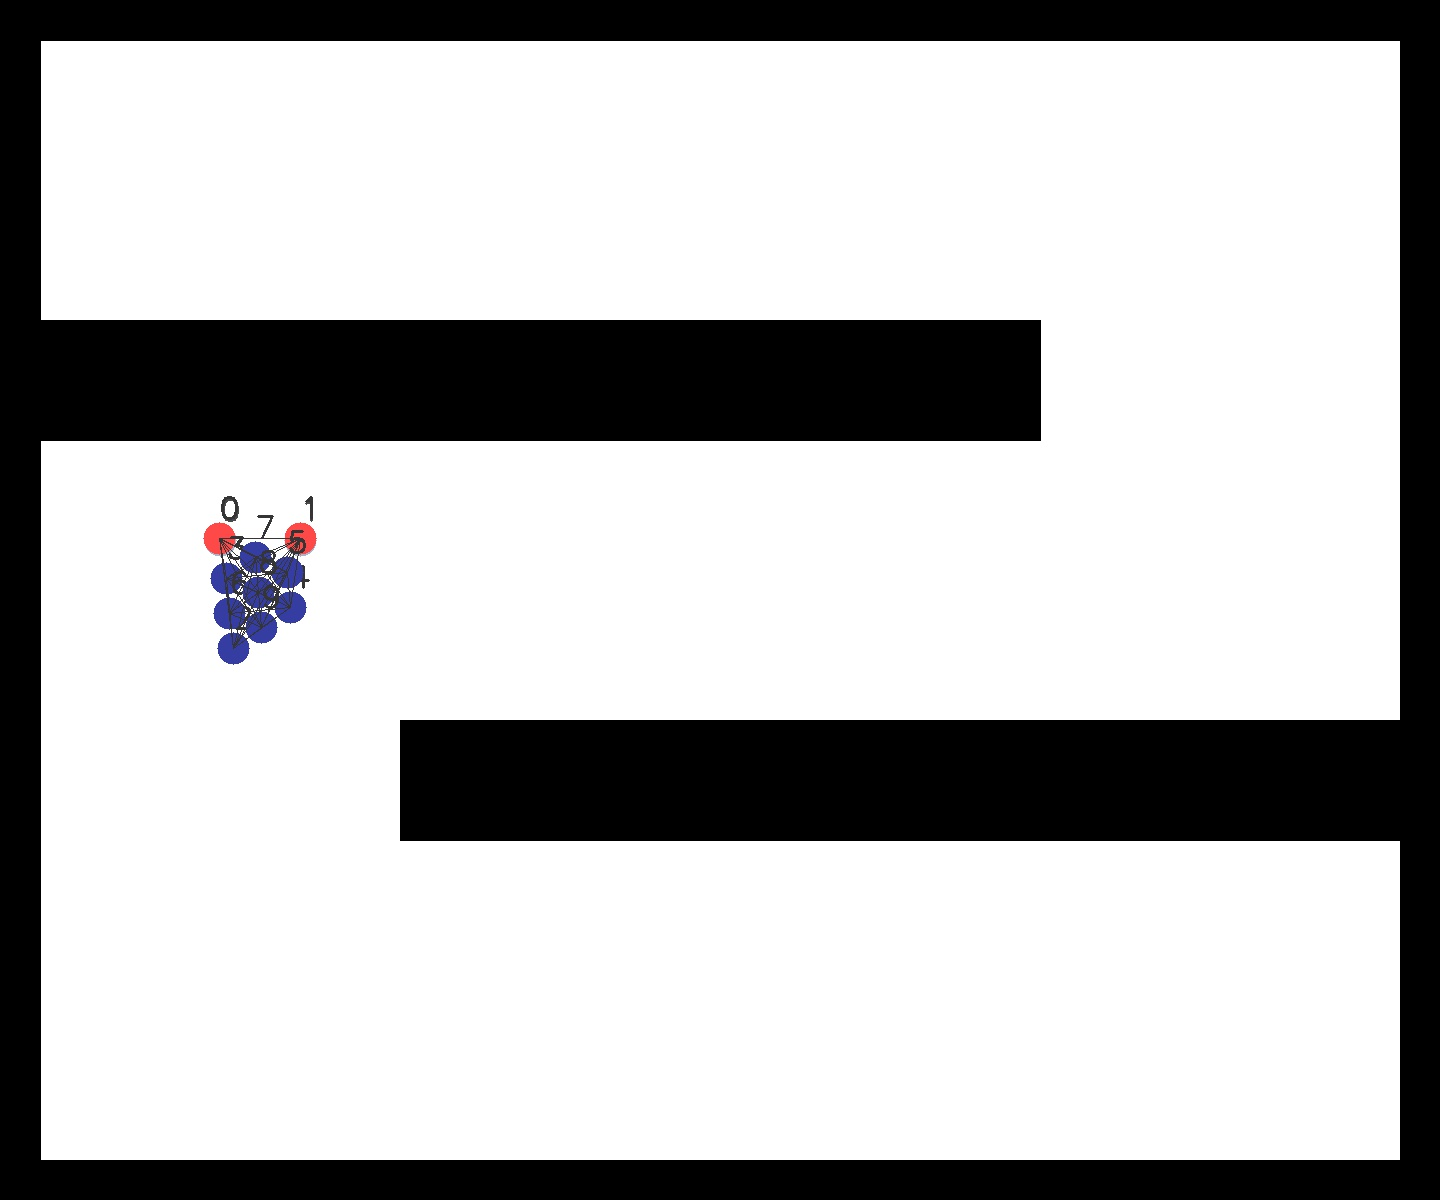
\includegraphics[width=\textwidth]{m3_mt3_2.jpg}
\caption{Task 3 Weighted Behavior Combination}
\label{fig:m3_mt3_2}
\end{subfigure} \hfill
\begin{subfigure}[b]{0.24\textwidth}
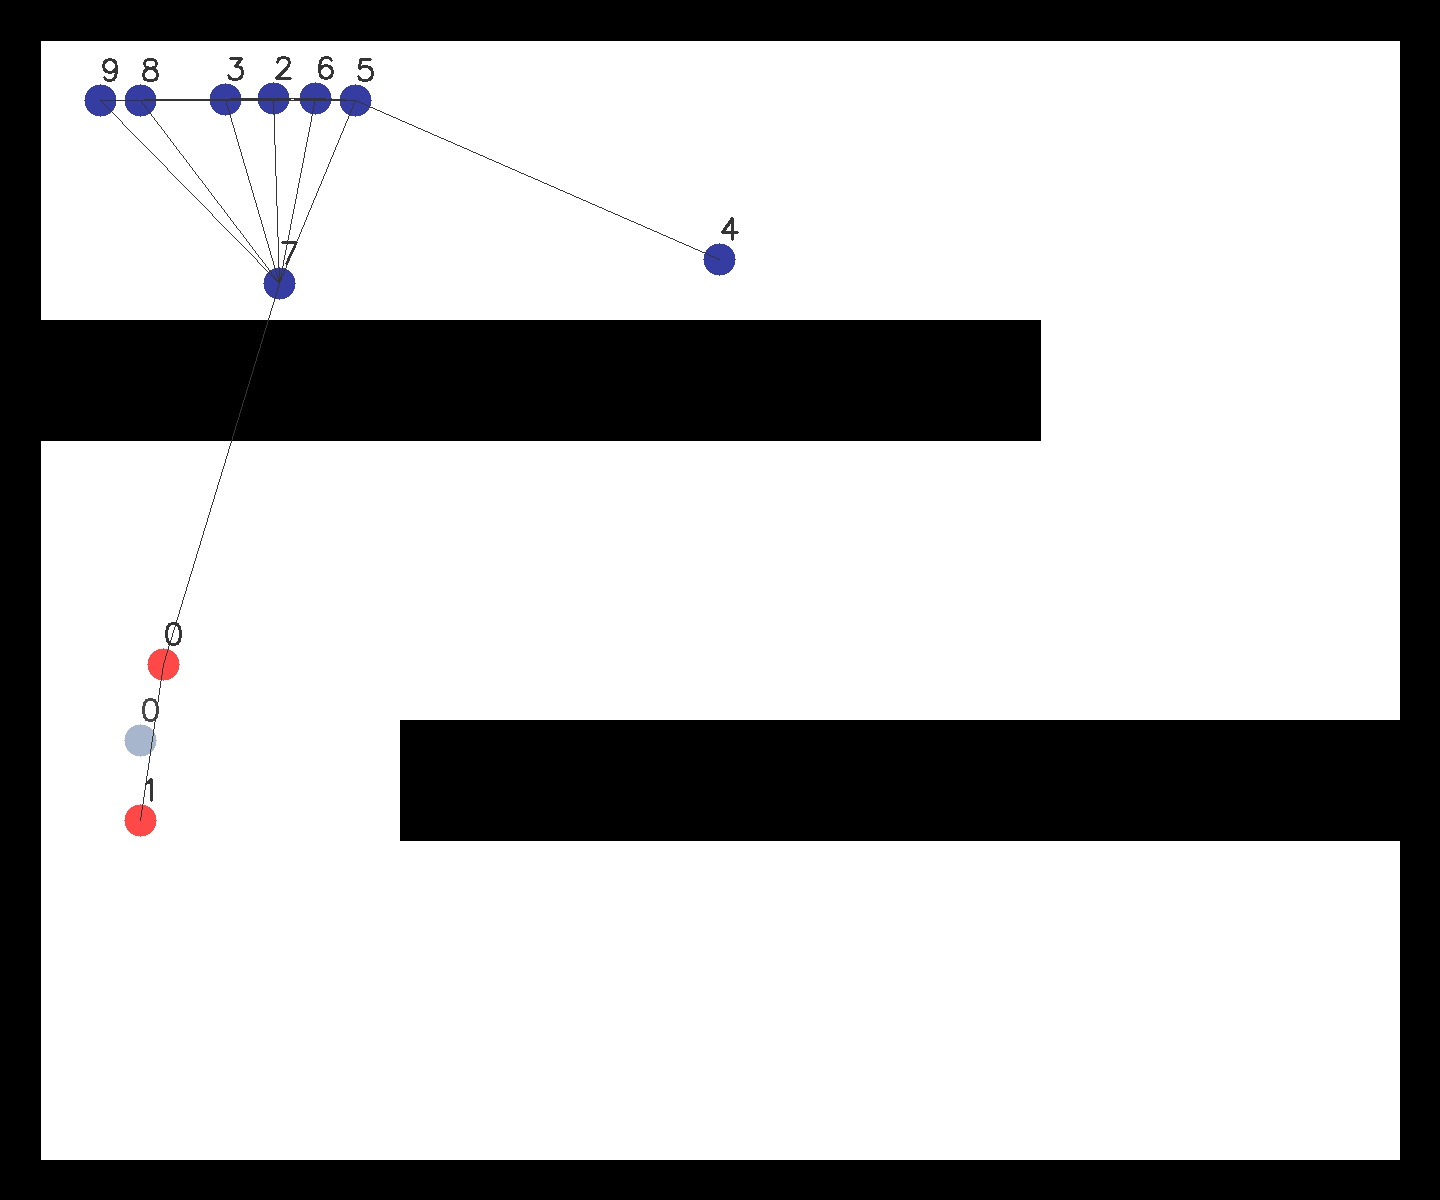
\includegraphics[width=\textwidth]{m3_mt0_1.jpg}
\caption{Task 2 No connection controller}
\label{fig:m3_mt0_1}
\end{subfigure}
\begin{subfigure}[b]{0.24\textwidth}
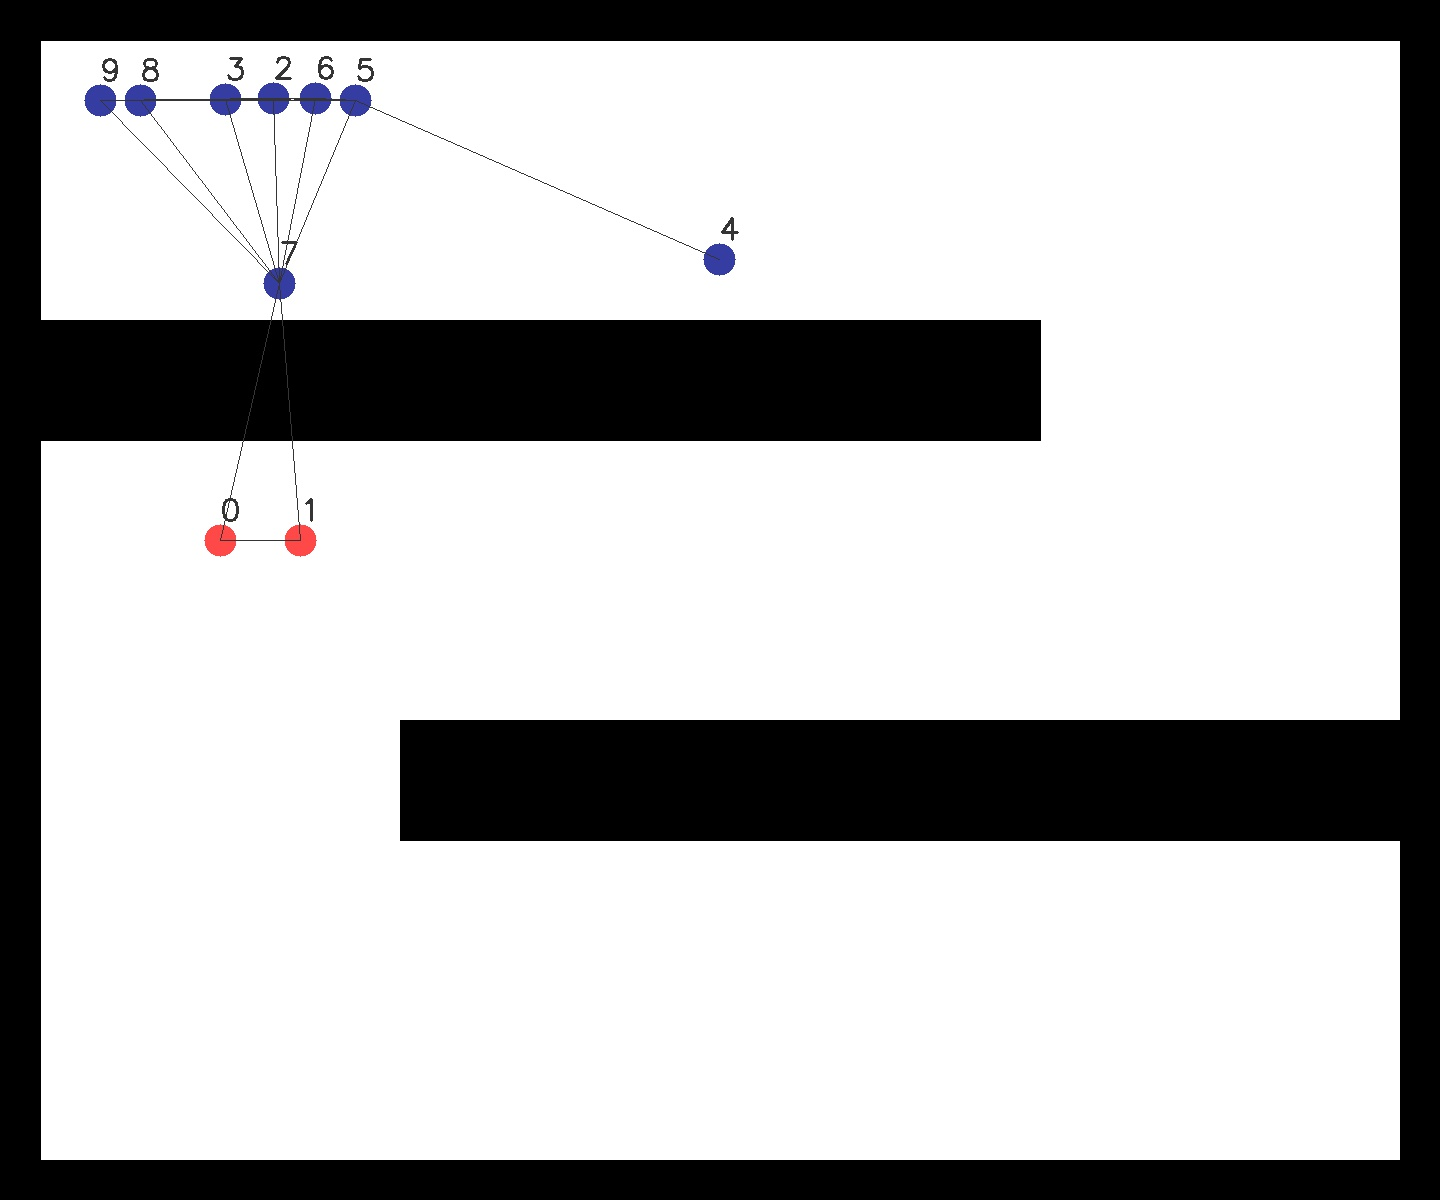
\includegraphics[width=\textwidth]{m3_mt0_2.jpg}
\caption{Task 3 No connection controller}
\label{fig:m3_mt0_2}
\end{subfigure} \\
\begin{subfigure}[b]{0.24\textwidth}
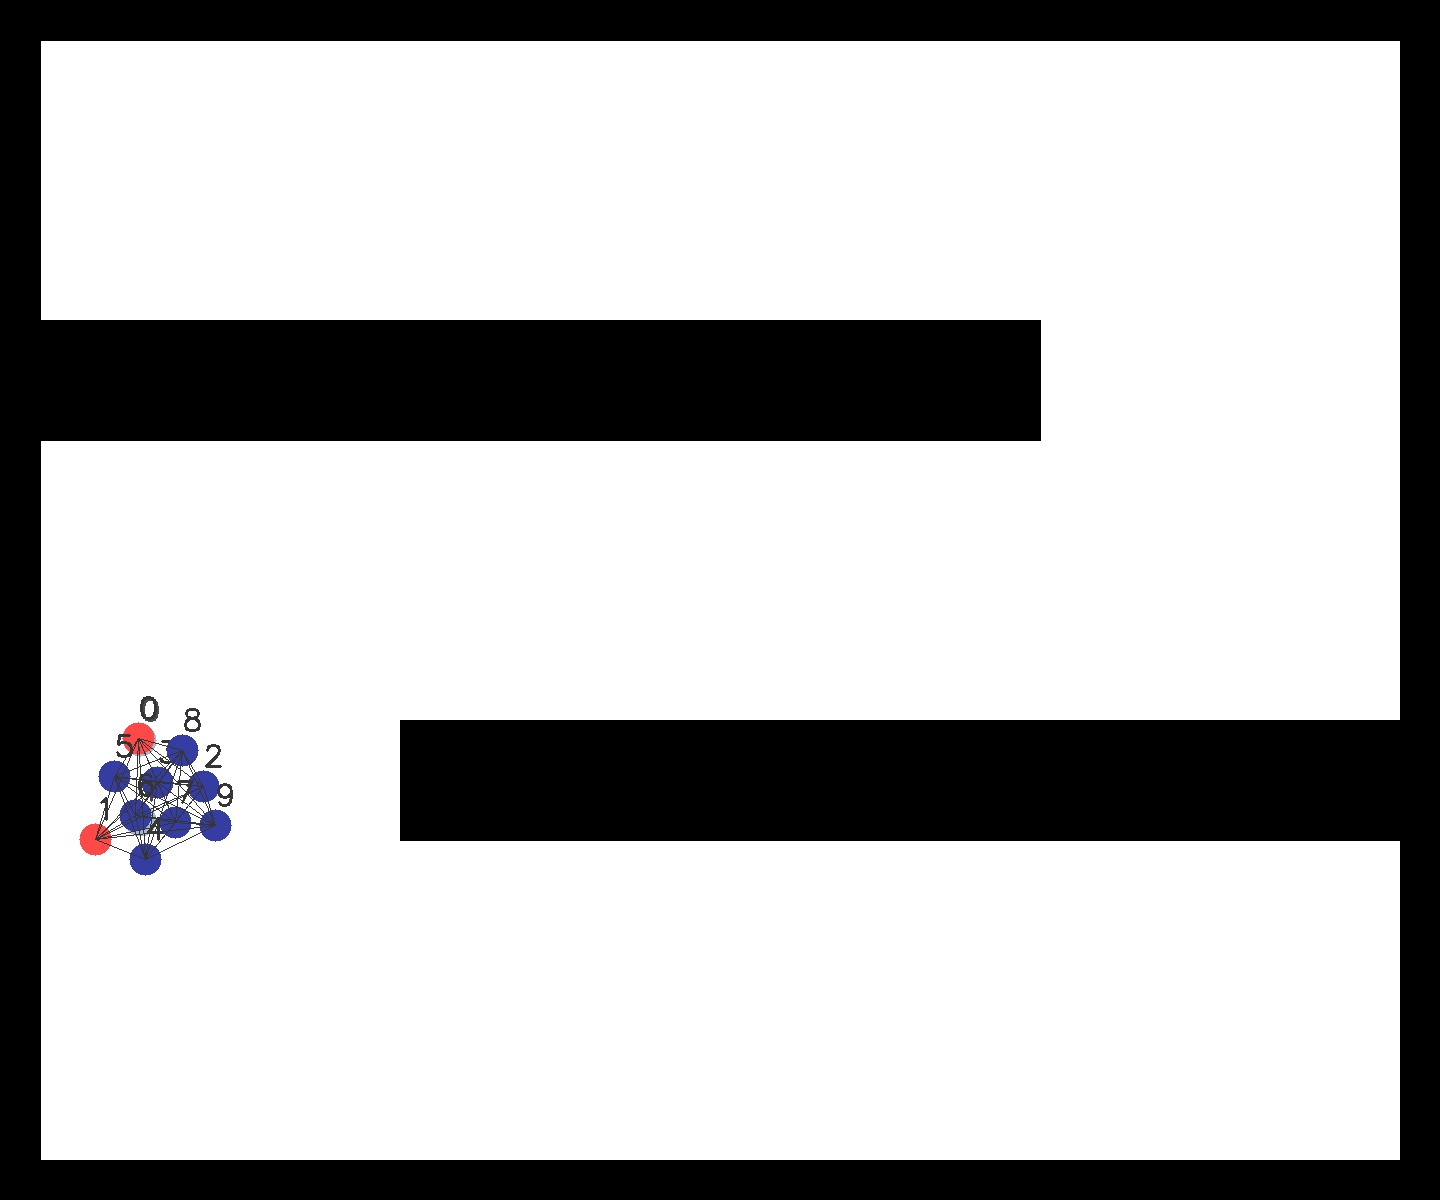
\includegraphics[width=\textwidth]{m3_mt1_1.jpg}
\caption{Task 2 Weighted Rendezvous}
\label{fig:m3_mt1_1}
\end{subfigure}
\begin{subfigure}[b]{0.24\textwidth}
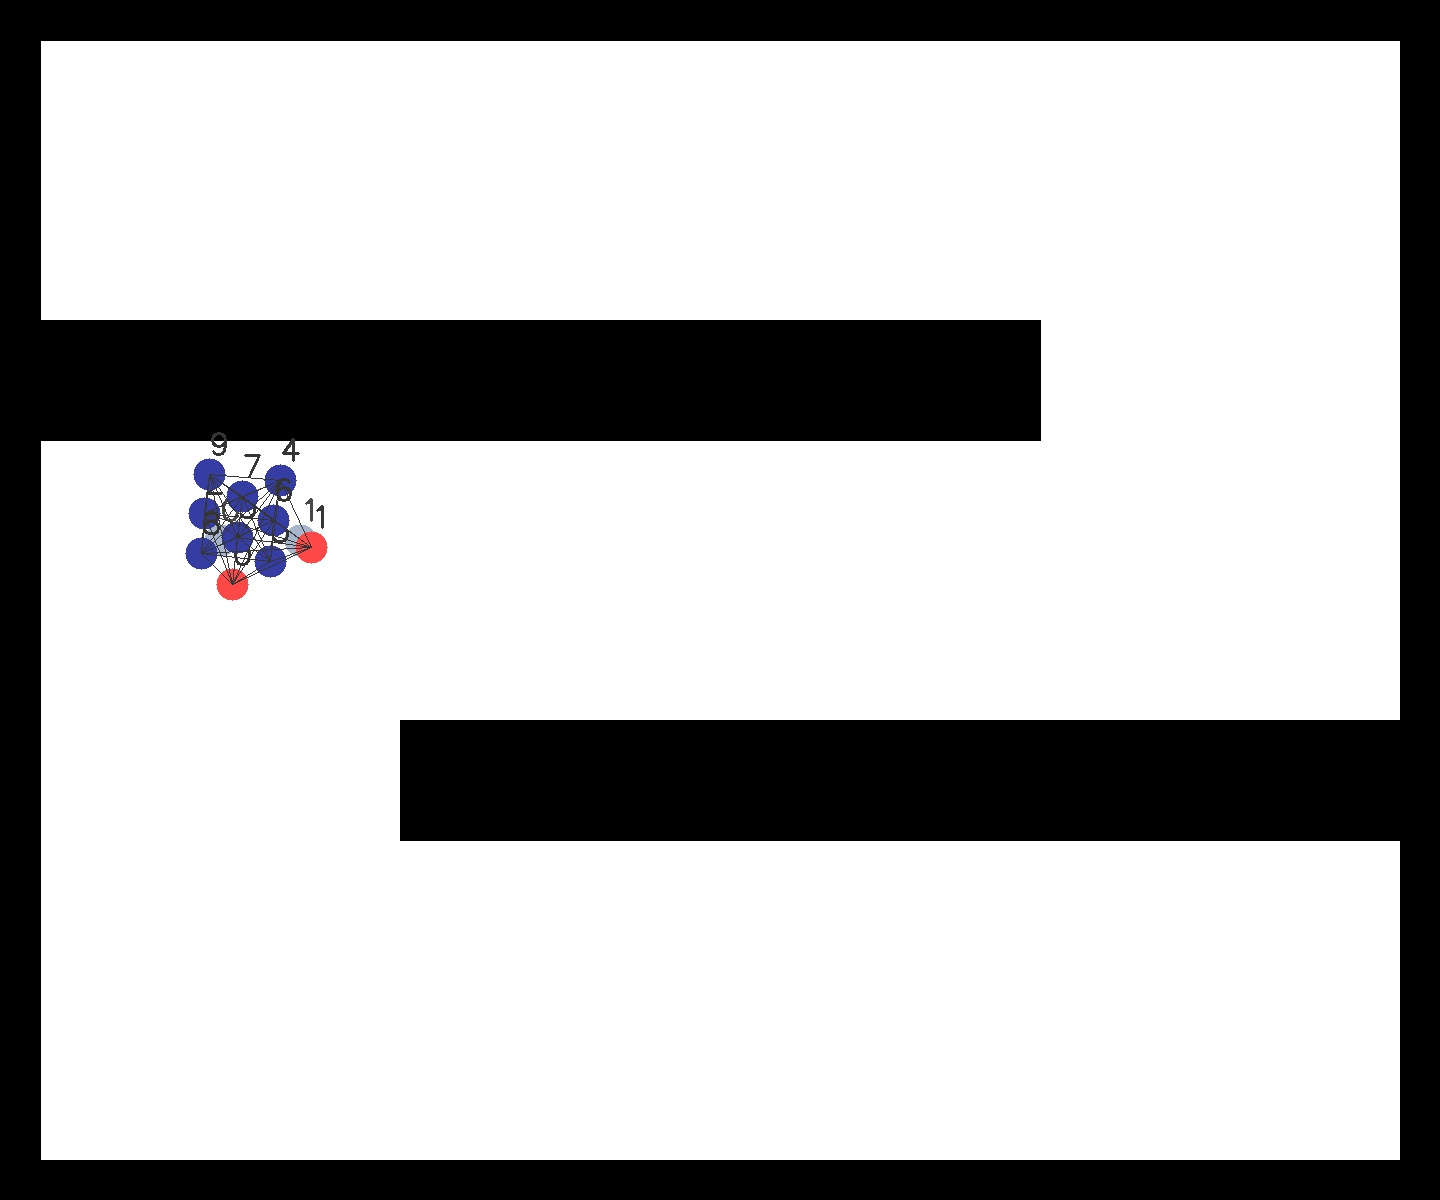
\includegraphics[width=\textwidth]{m3_mt1_2.jpg}
\caption{Task 3 Weighted Rendezvous}
\label{fig:m3_mt1_2}
\end{subfigure} \hfill
\begin{subfigure}[b]{0.24\textwidth}
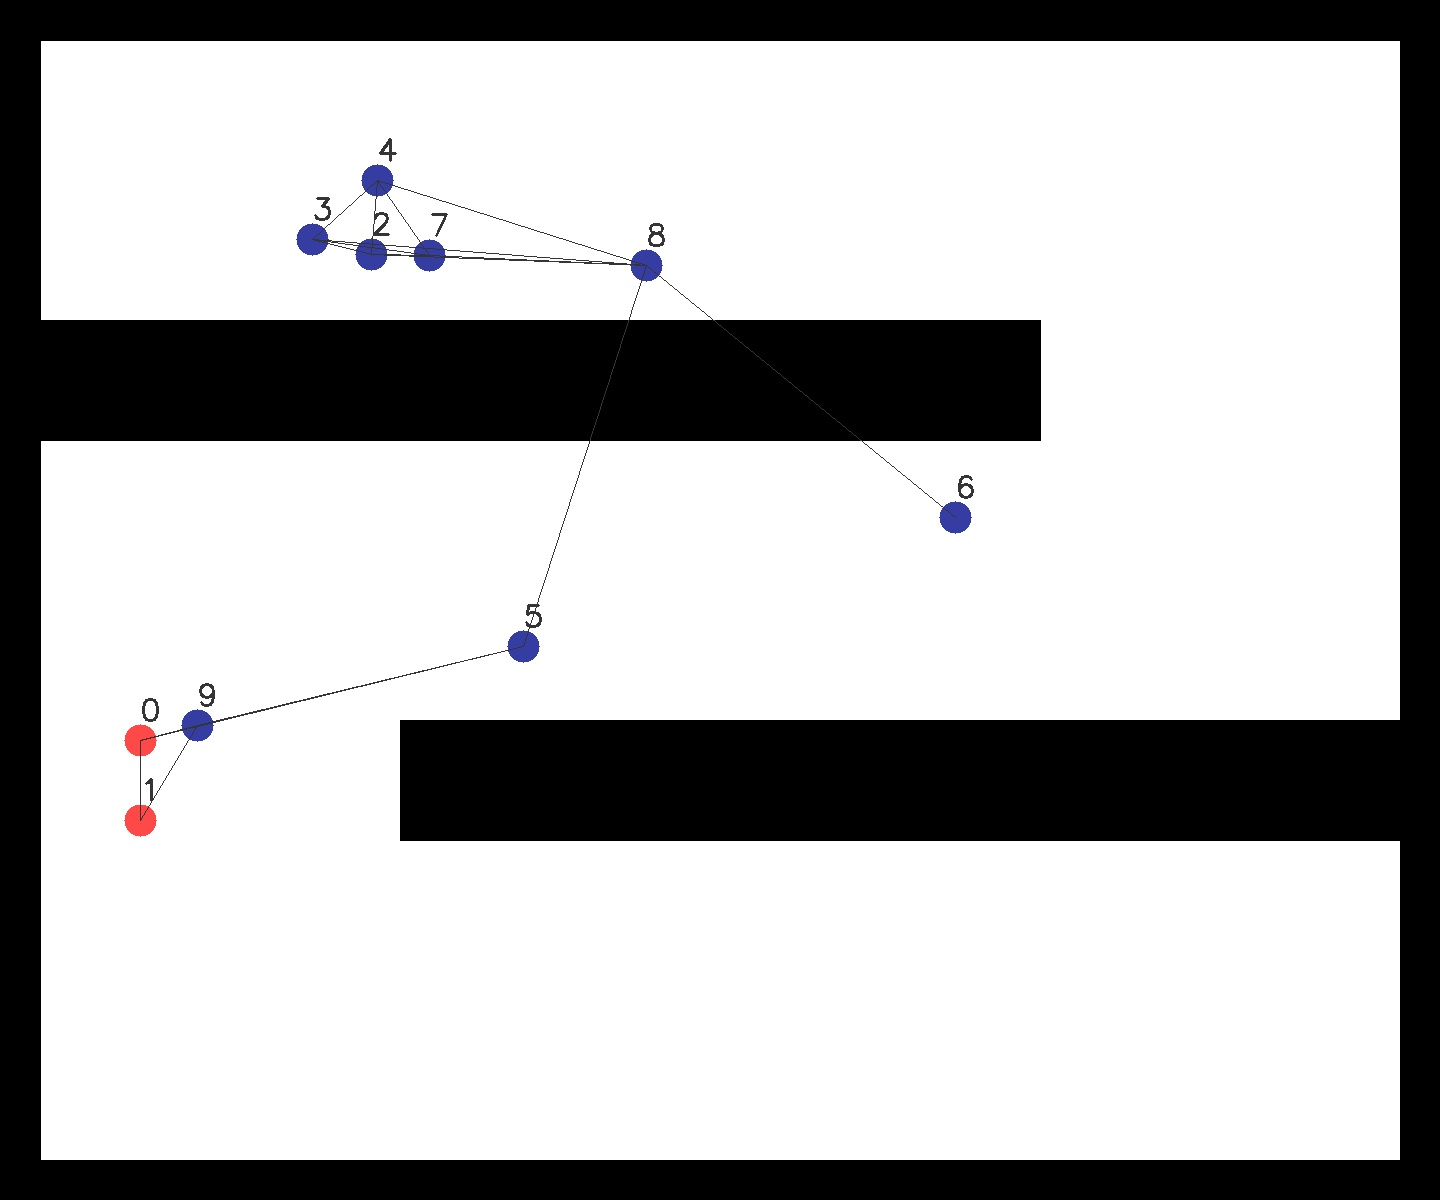
\includegraphics[width=\textwidth]{m3_mt2_1.jpg}
\caption{Task 2 Weighted Flocking}
\label{fig:m3_mt2_1}
\end{subfigure}
\begin{subfigure}[b]{0.24\textwidth}
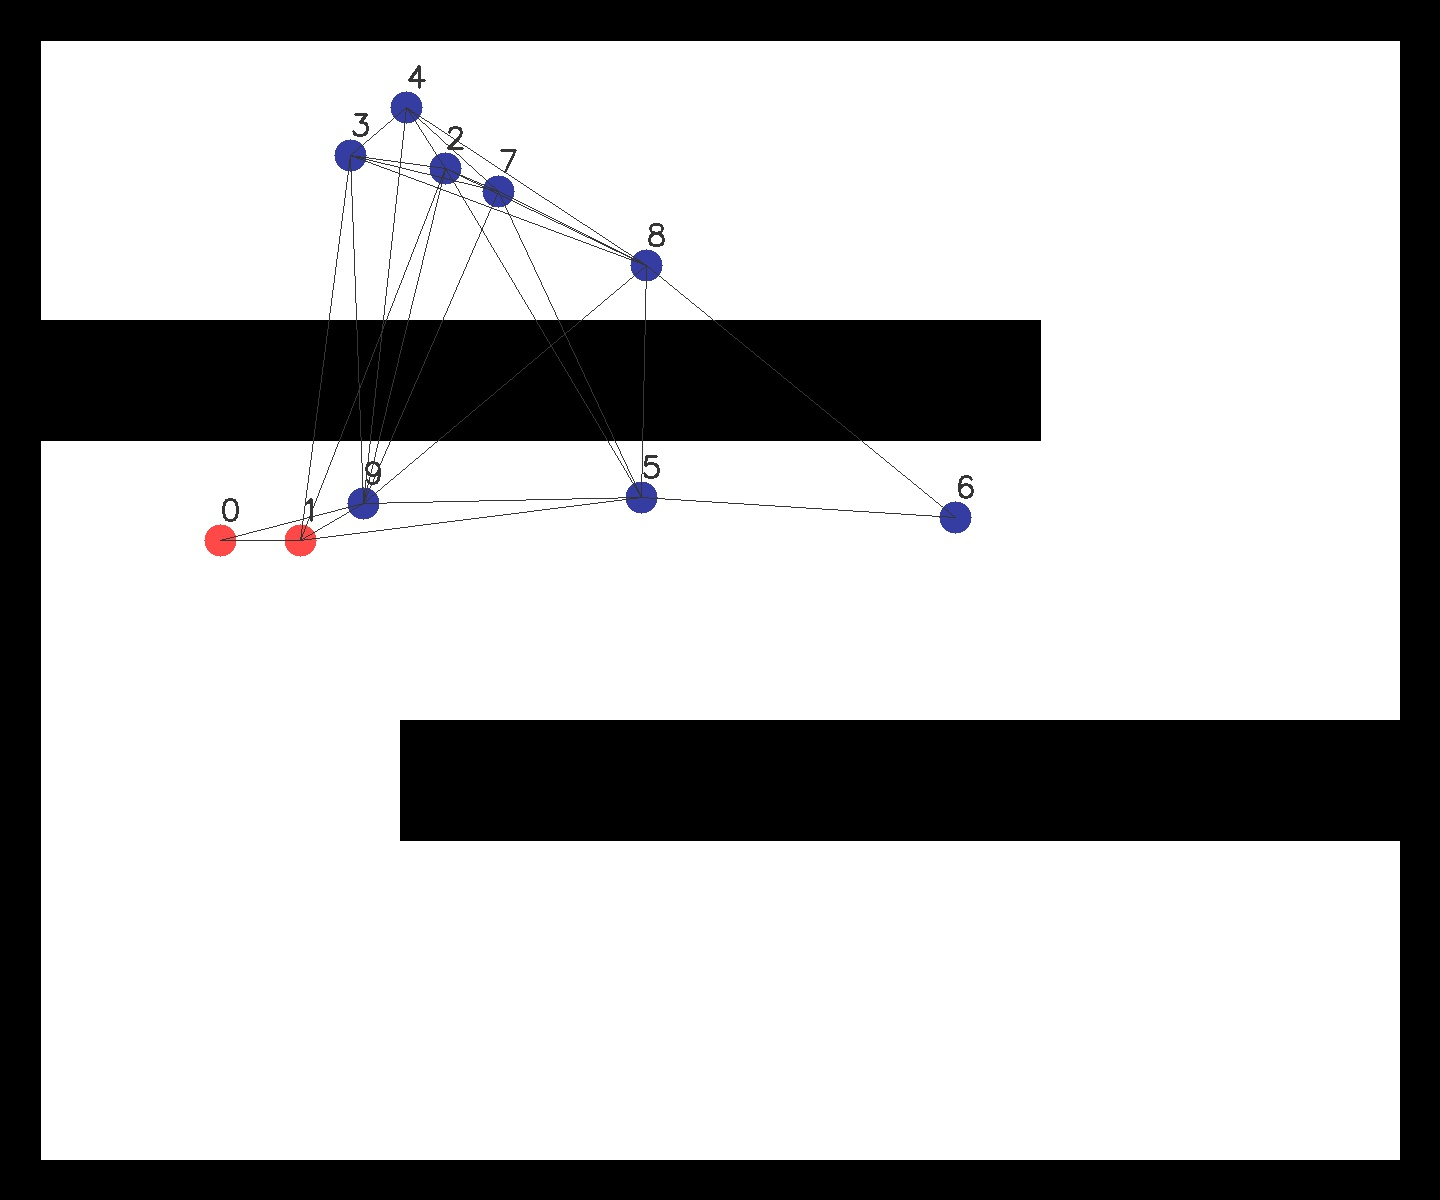
\includegraphics[width=\textwidth]{m3_mt2_2.jpg}
\caption{Task 3 Weighted Flocking}
\label{fig:m3_mt2_2}
\end{subfigure} \\
\begin{subfigure}[b]{0.24\textwidth}
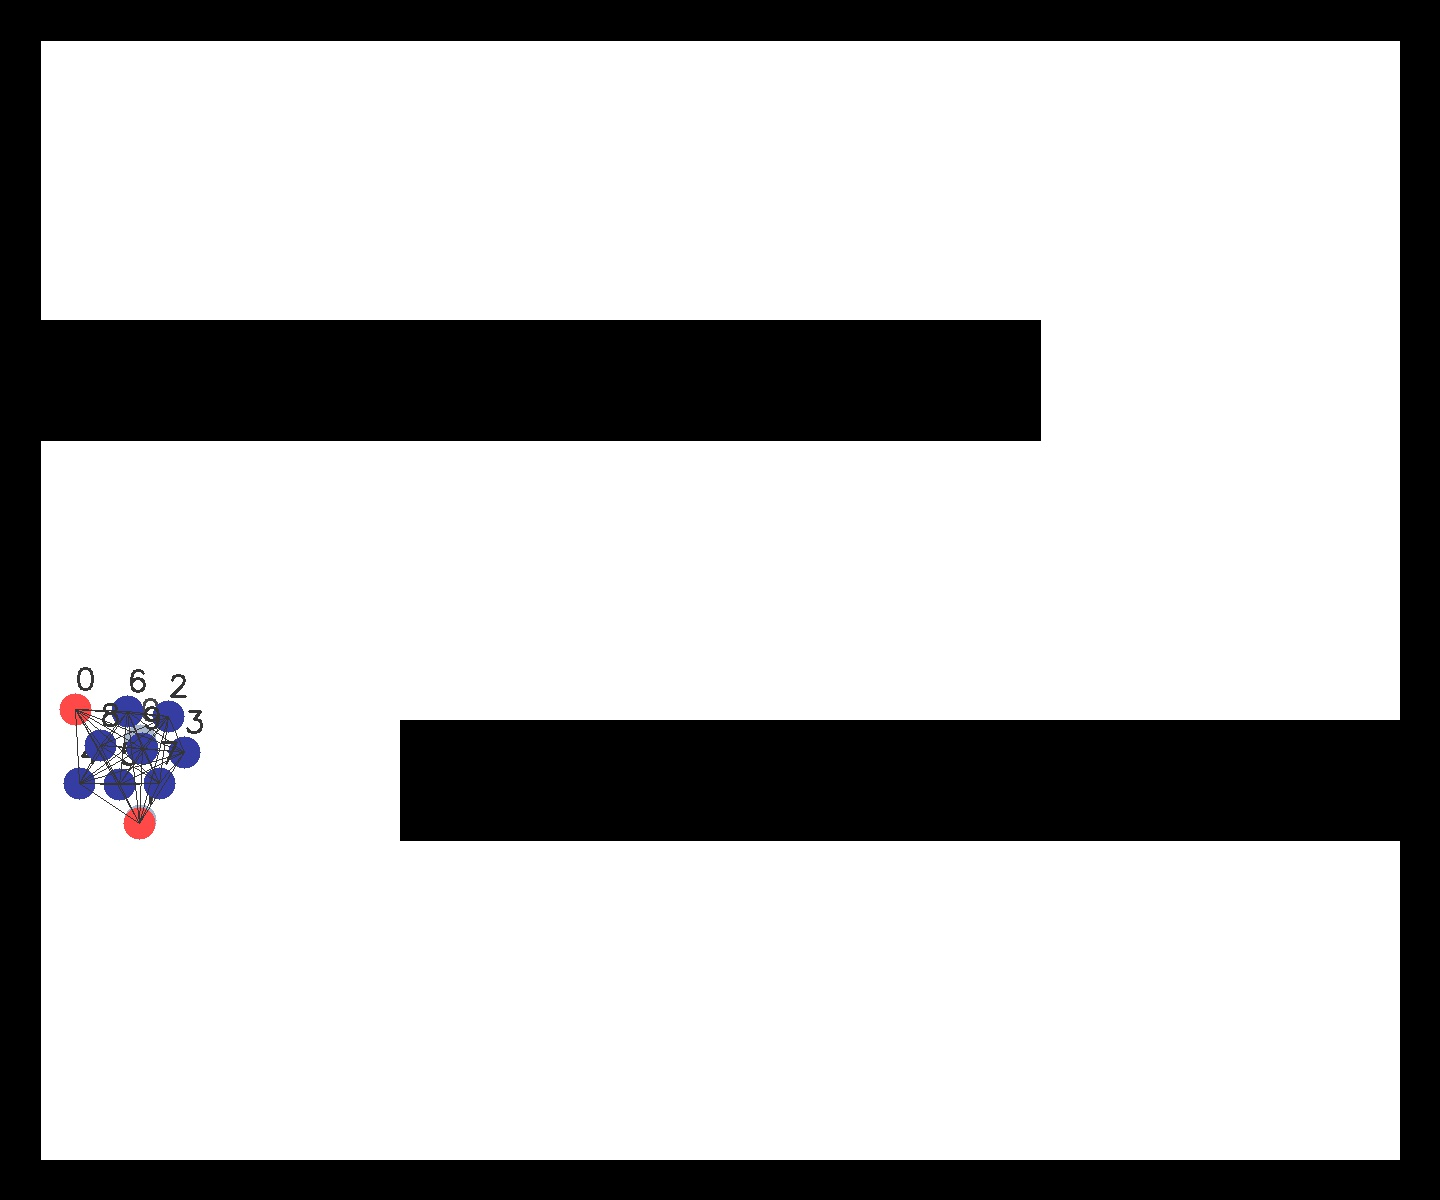
\includegraphics[width=\textwidth]{m3_mt4_1.jpg}
\caption{Task 2 Rendezvous}
\label{fig:m3_mt4_1}
\end{subfigure}
\begin{subfigure}[b]{0.24\textwidth}
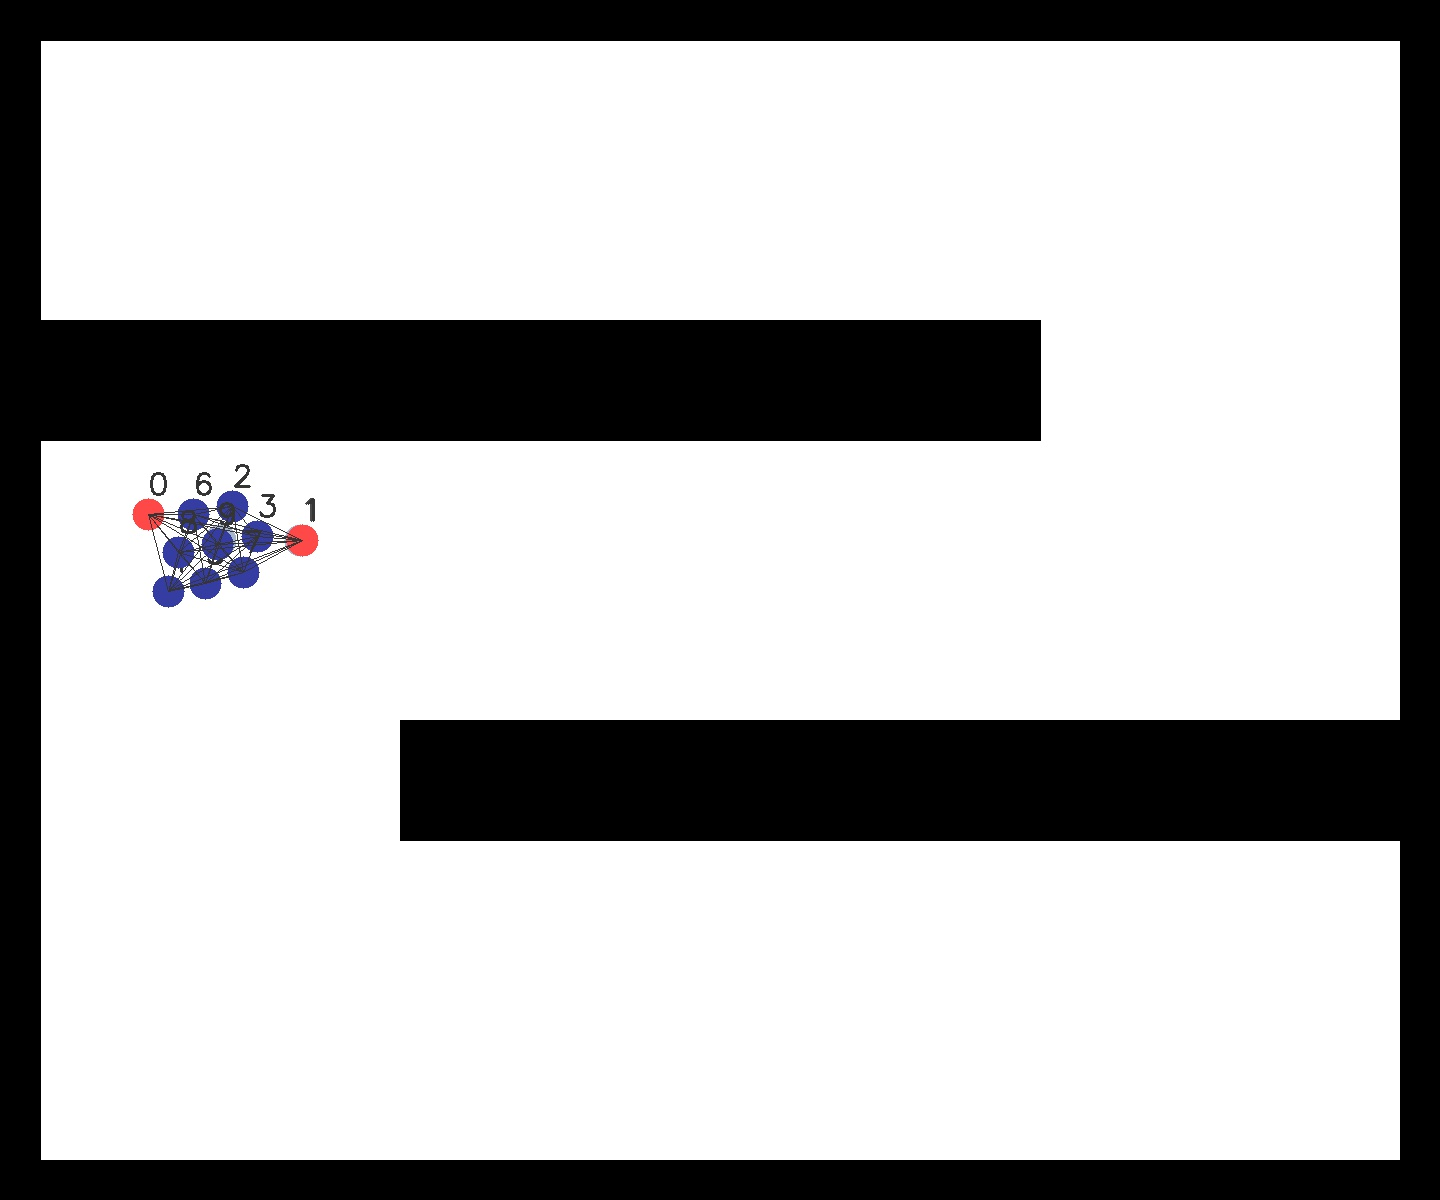
\includegraphics[width=\textwidth]{m3_mt4_2.jpg}
\caption{Task 3 Rendezvous}
\label{fig:m3_mt4_2}
\end{subfigure}
\caption{Red robots: task robots, blue robots: connection robots, light blue circles: goal locations. The process of $N=10$ robots executing task 2 and 3 in Map~\ref{fig:map_1} with no connection controller. (a)-(b) Weighted behavior combination: the task robots are able to reach all the goal locations and the connection robots are able to keep up with the task robots till the end; (c)-(d) No connection controller: robot failing the task due to connectivity constraints; (e)-(f) Weighted rendezvous: connection robots blocking the task robots; (g)-(h) Weighted flocking: some robots were left behind; (i)-(j) Rendezvous: connection robots blocking the task robots.}
\label{fig:m3}
\end{figure}

\begin{figure}
\centering
\begin{subfigure}[b]{0.24\textwidth}
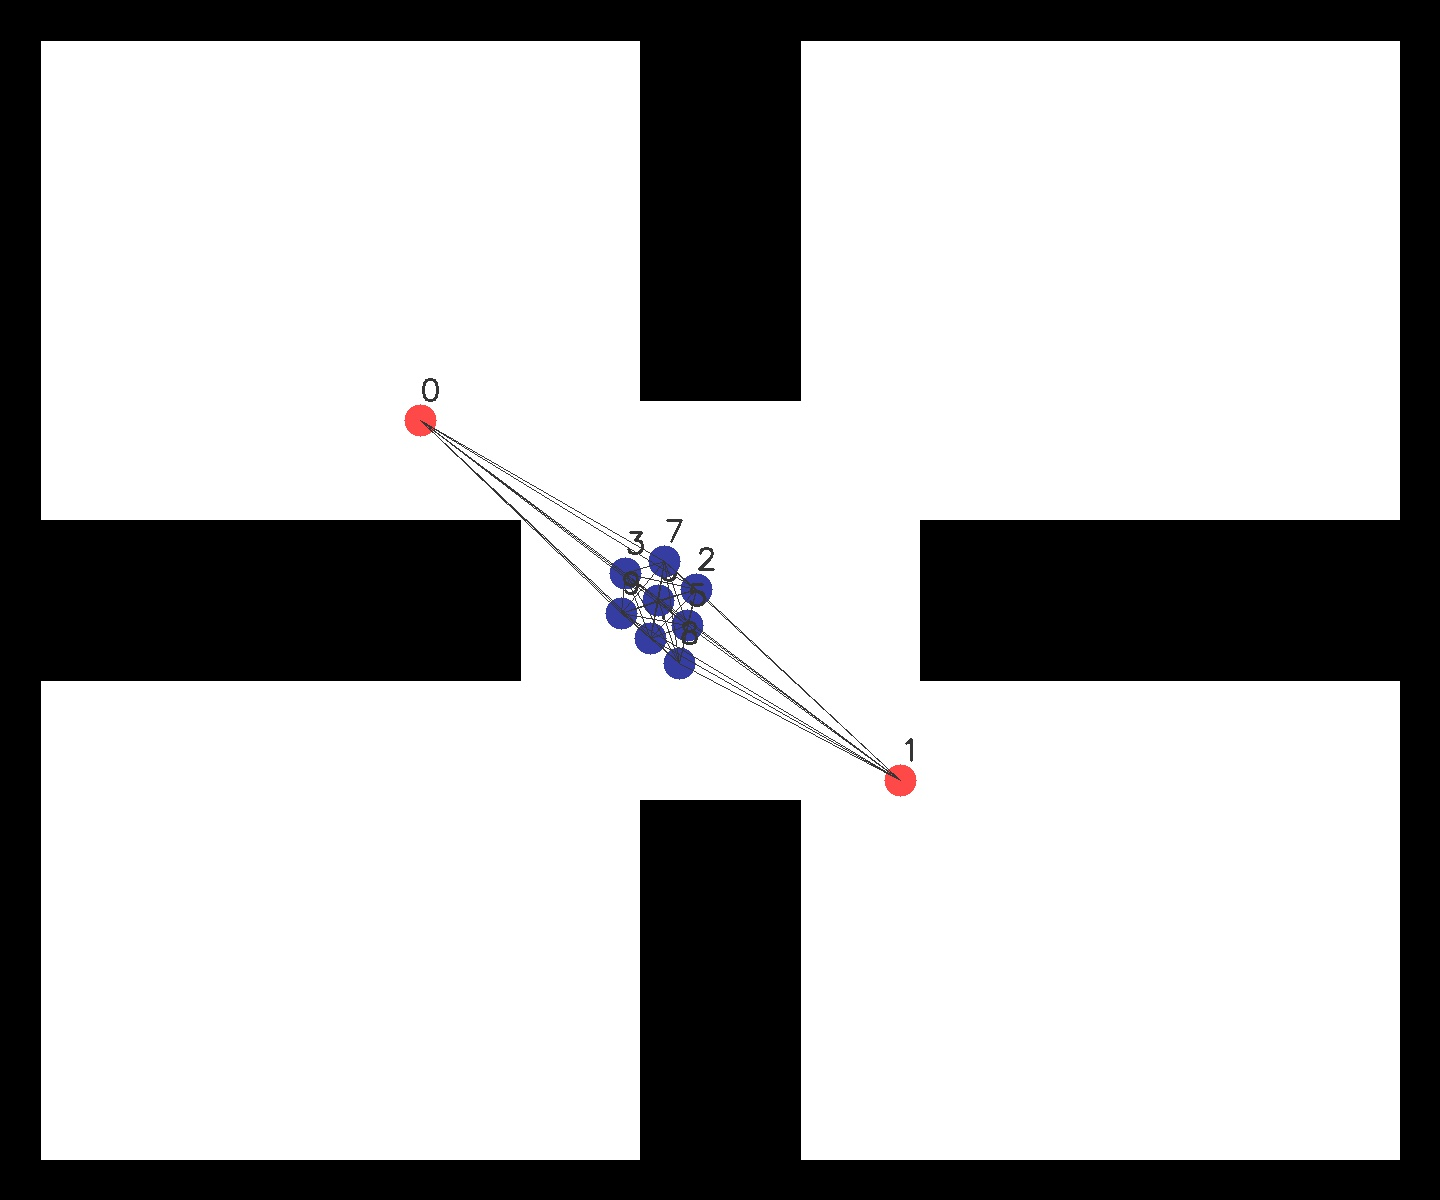
\includegraphics[width=\textwidth]{m4_mt3_0.jpg}
\caption{Task 1 Weighted Behavior Combination}
\label{fig:m4_mt3_0}
\end{subfigure}
\begin{subfigure}[b]{0.24\textwidth}
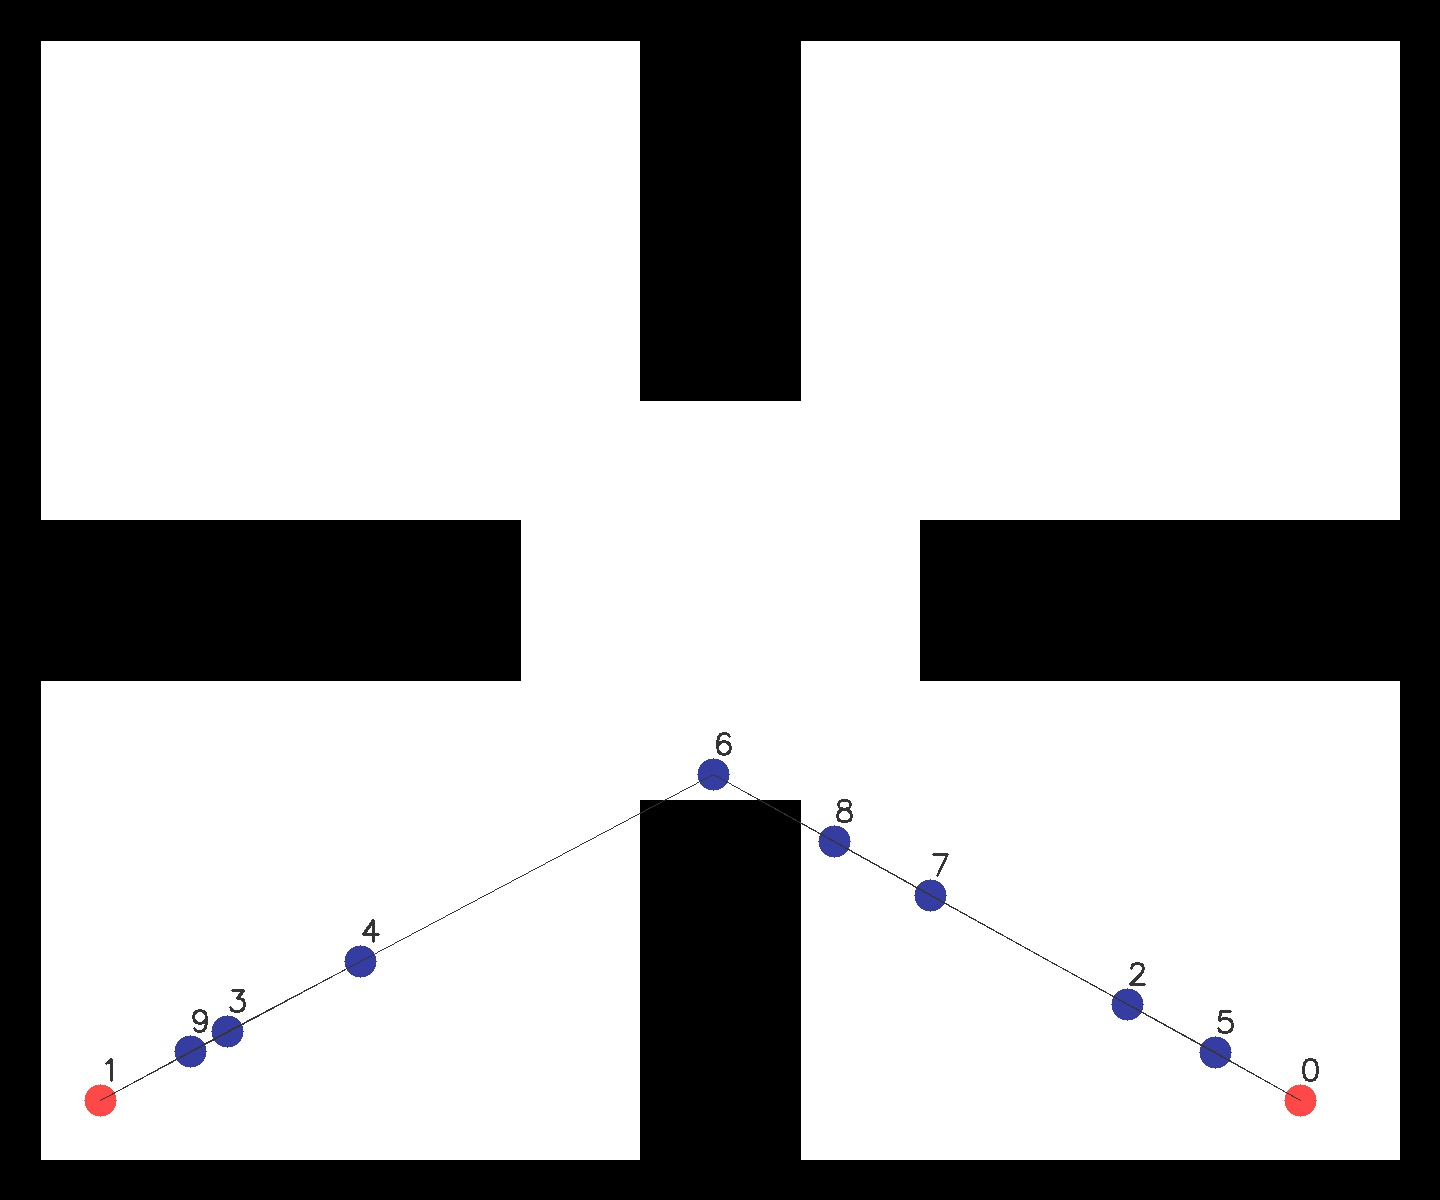
\includegraphics[width=\textwidth]{m4_mt3_2.jpg}
\caption{Task 3 Weighted Behavior Combination}
\label{fig:m4_mt3_2}
\end{subfigure} \hfill
\begin{subfigure}[b]{0.24\textwidth}
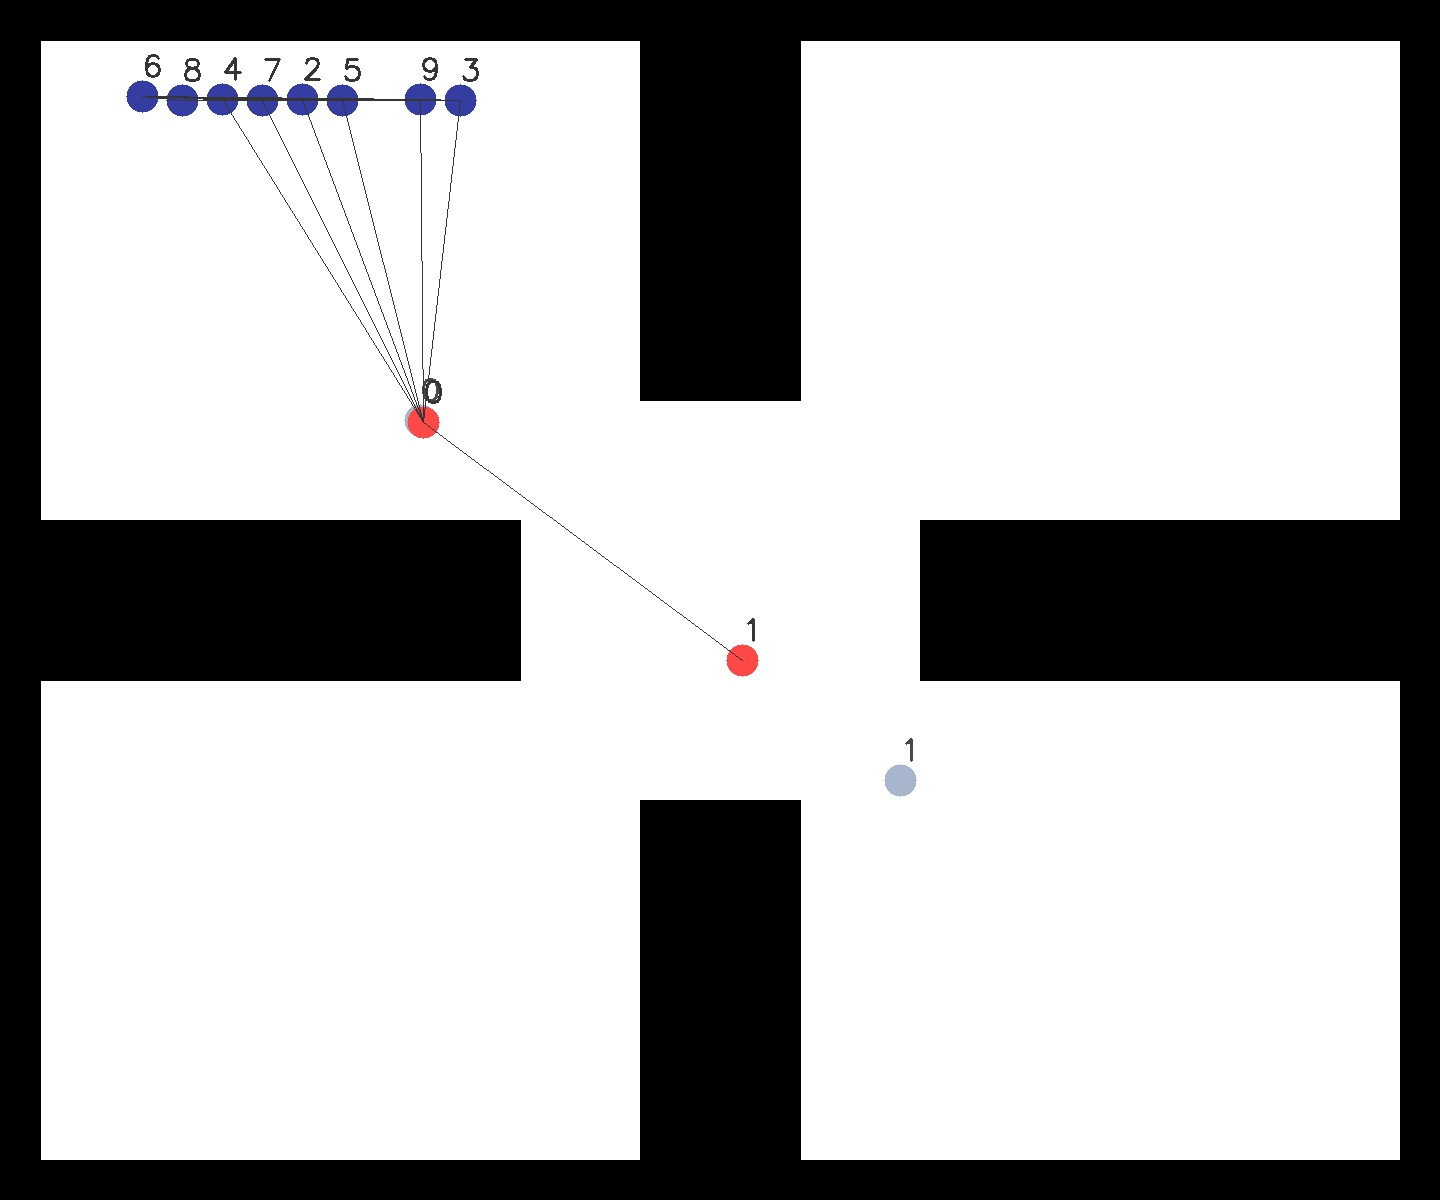
\includegraphics[width=\textwidth]{m4_mt0_0.jpg}
\caption{Task 1 No connection controller}
\label{fig:m4_mt0_0}
\end{subfigure}
\begin{subfigure}[b]{0.24\textwidth}
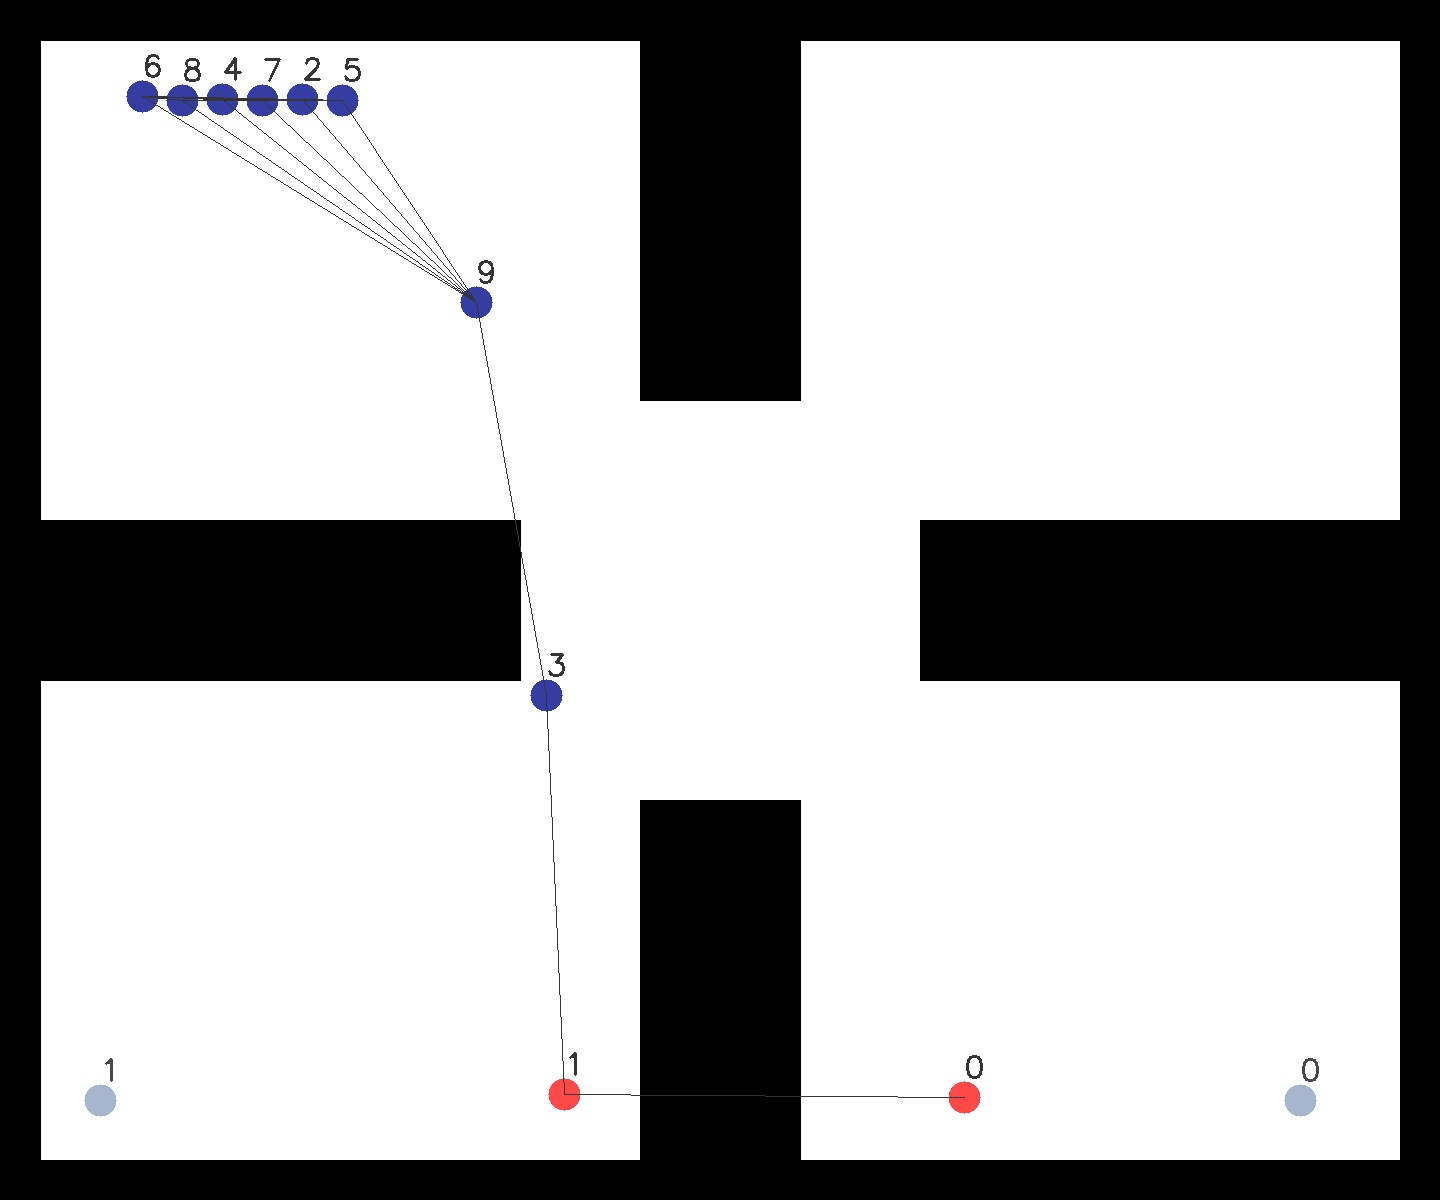
\includegraphics[width=\textwidth]{m4_mt0_2.jpg}
\caption{Task 3 No connection controller}
\label{fig:m4_mt0_2}
\end{subfigure} \\
\begin{subfigure}[b]{0.24\textwidth}
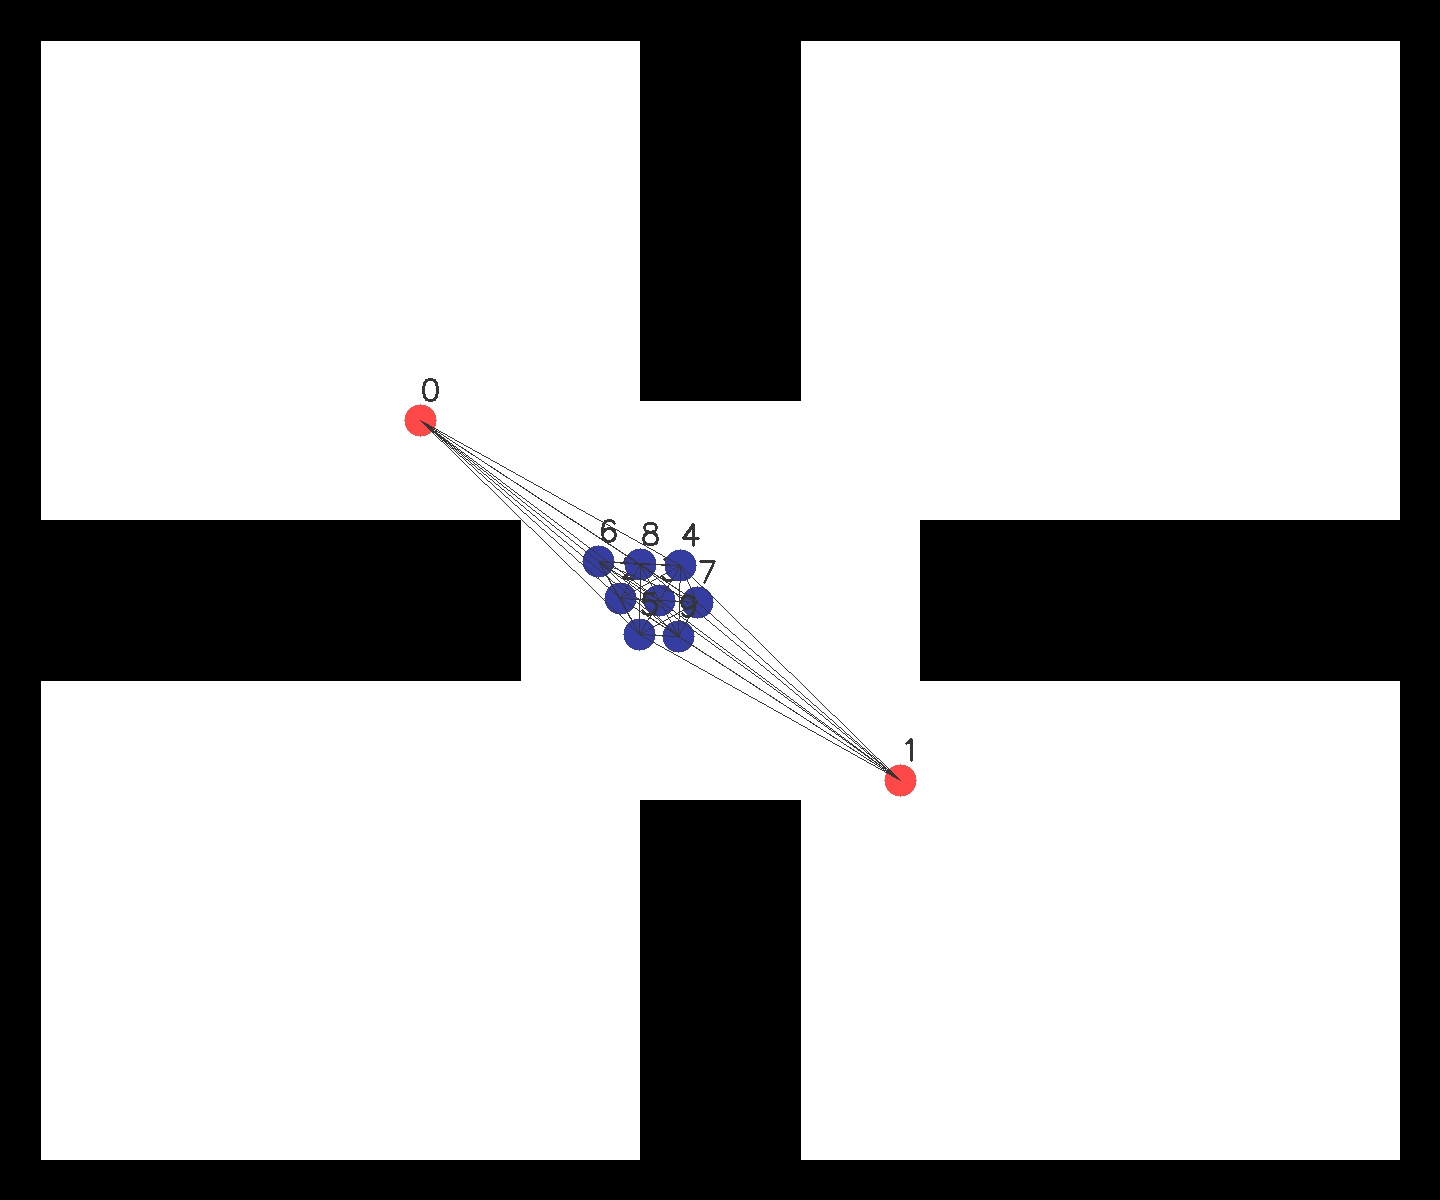
\includegraphics[width=\textwidth]{m4_mt1_0.jpg}
\caption{Task 1 Weighted Rendezvous}
\label{fig:m4_mt1_0}
\end{subfigure}
\begin{subfigure}[b]{0.24\textwidth}
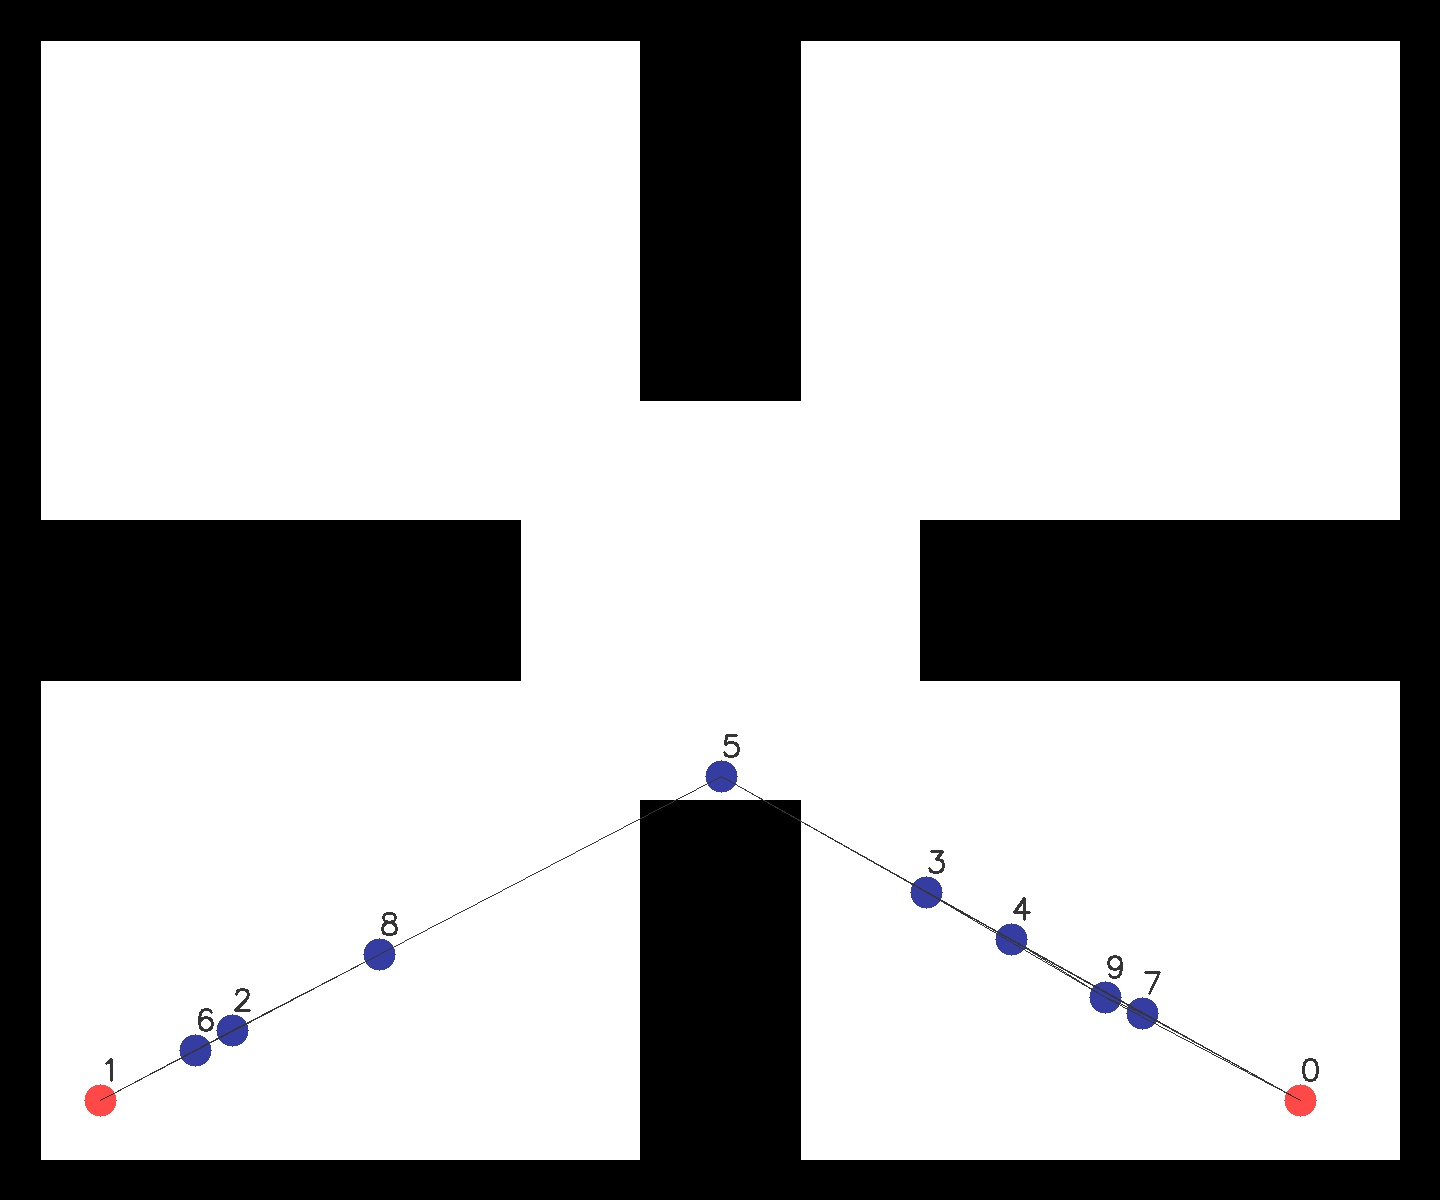
\includegraphics[width=\textwidth]{m4_mt1_2.jpg}
\caption{Task 3 Weighted Rendezvous}
\label{fig:m4_mt1_2}
\end{subfigure} \hfill
\begin{subfigure}[b]{0.24\textwidth}
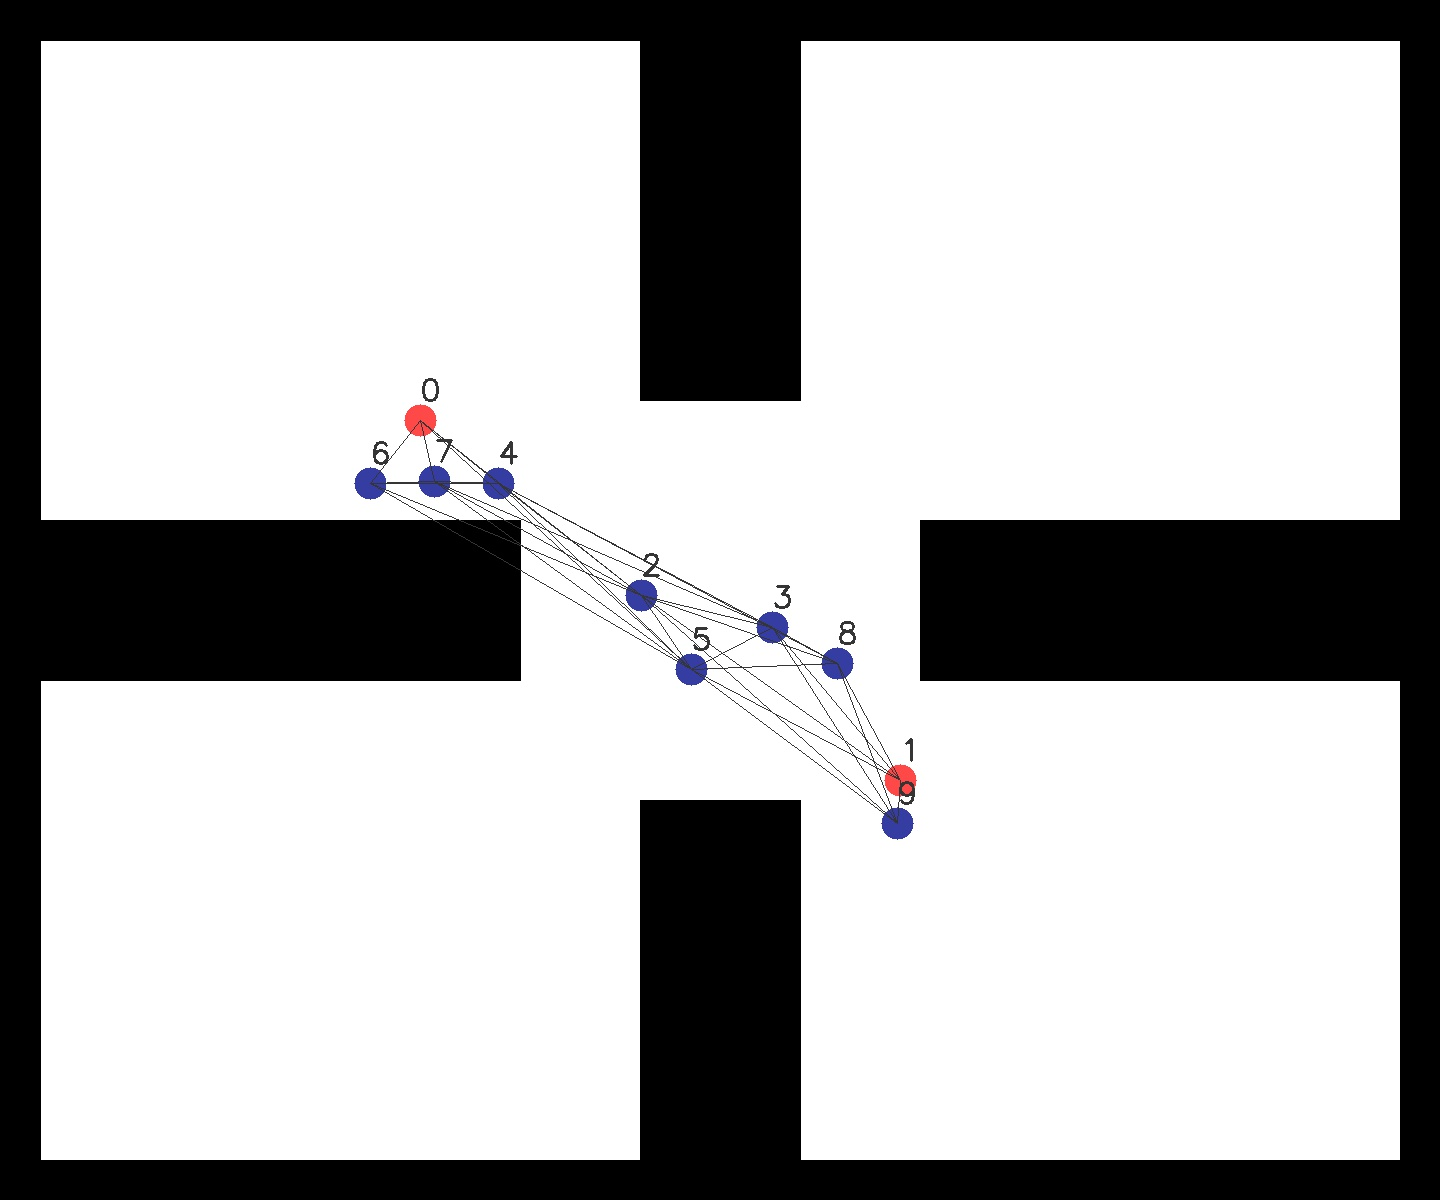
\includegraphics[width=\textwidth]{m4_mt2_0.jpg}
\caption{Task 1 Weighted Flocking}
\label{fig:m4_mt2_0}
\end{subfigure}
\begin{subfigure}[b]{0.24\textwidth}
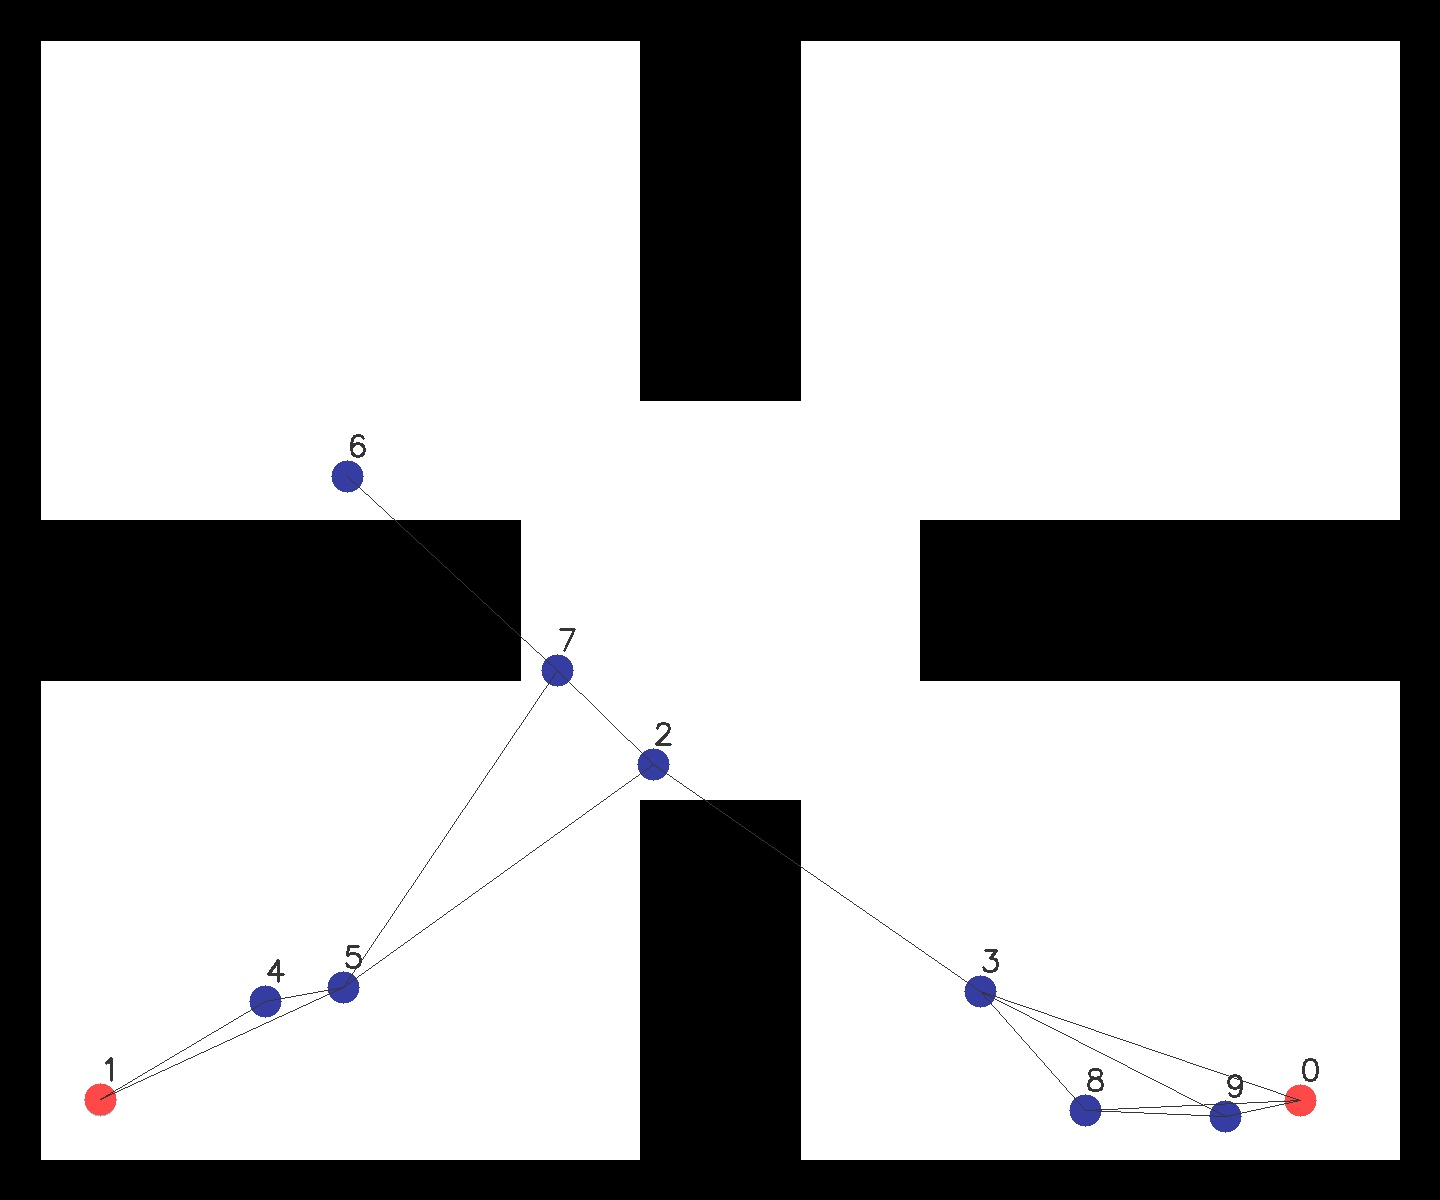
\includegraphics[width=\textwidth]{m4_mt2_2.jpg}
\caption{Task 3 Weighted Flocking}
\label{fig:m4_mt2_2}
\end{subfigure} \\
\begin{subfigure}[b]{0.24\textwidth}
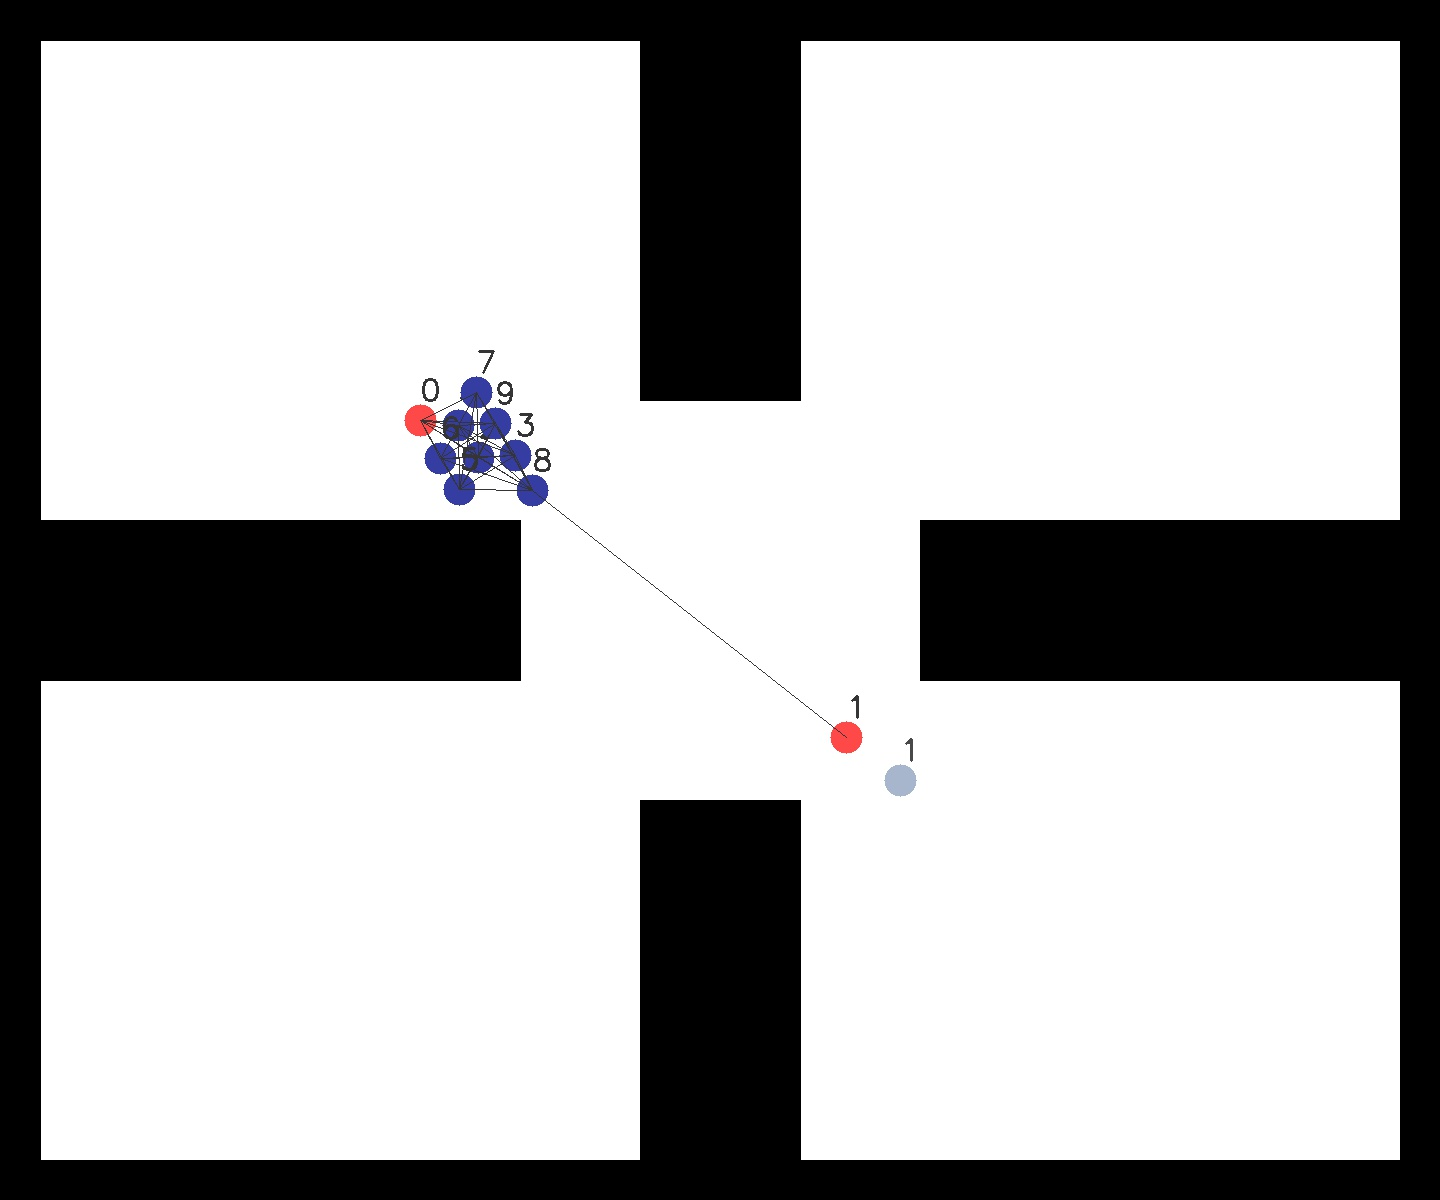
\includegraphics[width=\textwidth]{m4_mt4_0.jpg}
\caption{Task 1 Rendezvous}
\label{fig:m4_mt4_0}
\end{subfigure}
\begin{subfigure}[b]{0.24\textwidth}
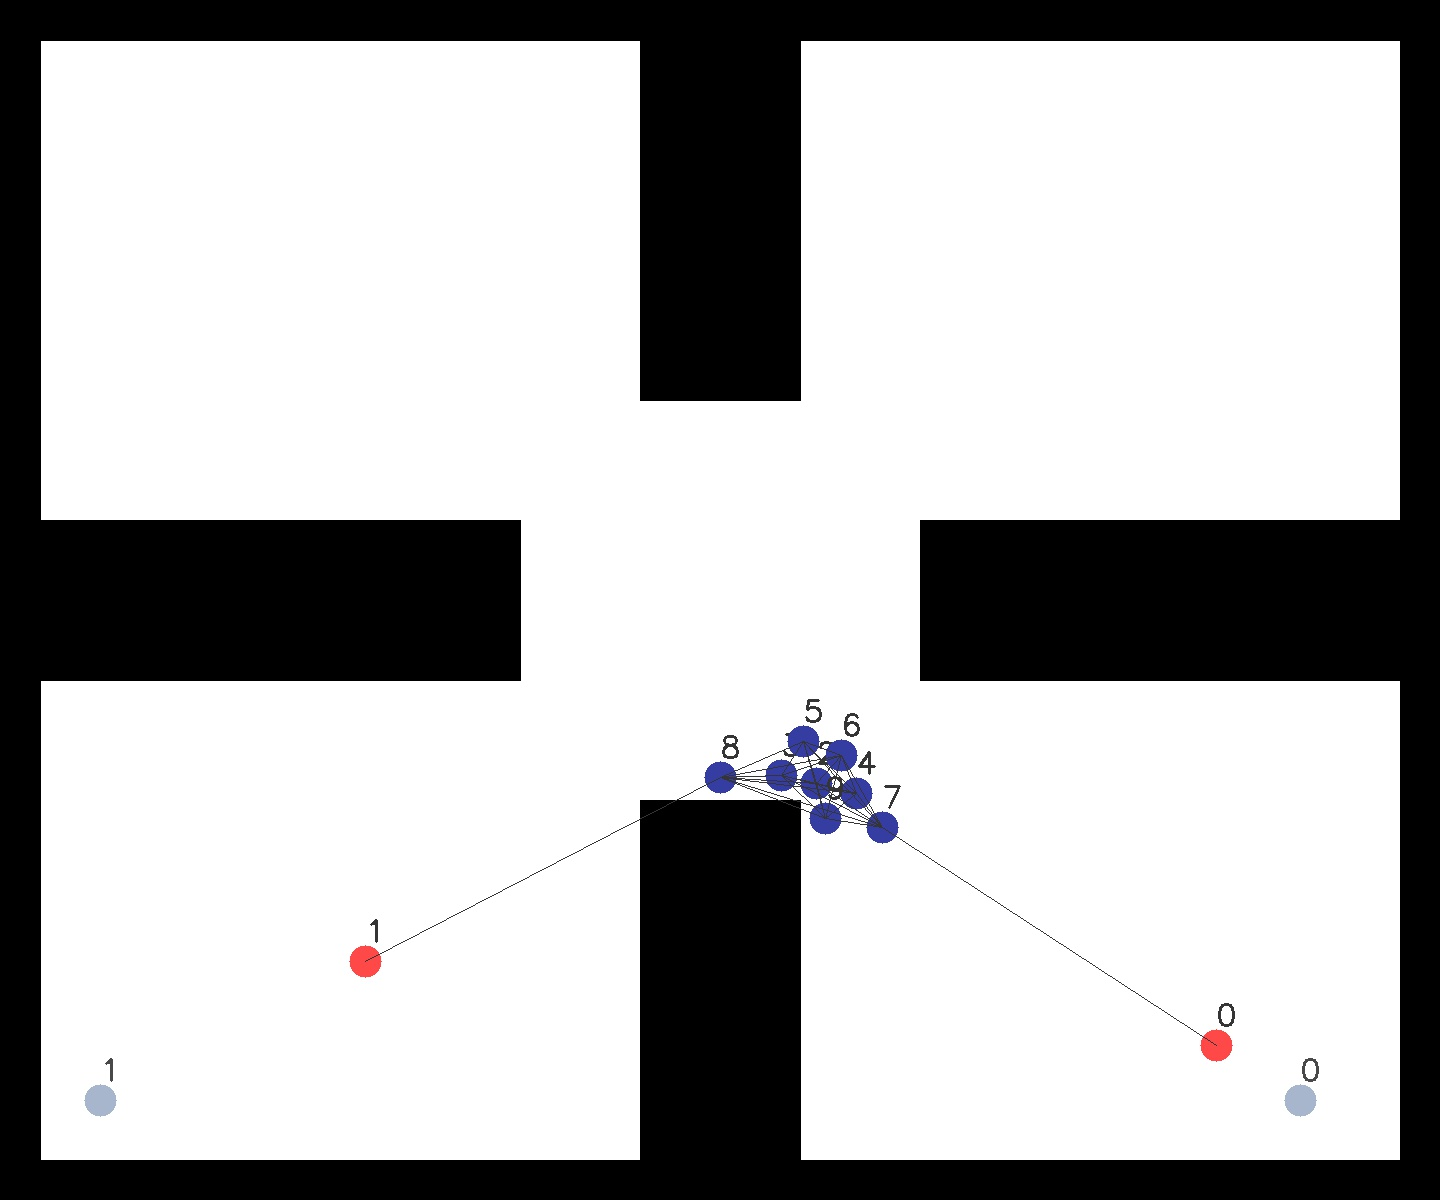
\includegraphics[width=\textwidth]{m4_mt4_2.jpg}
\caption{Task 3 Rendezvous}
\label{fig:m4_mt4_2}
\end{subfigure}
\setlength{\belowcaptionskip}{-14pt}
\caption{Red robots: task robots, blue robots: connection robots, light blue circles: goal locations. The process of $N=10$ robots executing task 1 and 3 in Map~\ref{fig:map_2} with no connection controller. (a)-(b) Weighted behavior combination: the task robots are able to reach all the goal locations and the connection robots are able to keep up with the task robots till the end; (c)-(d) No connection controller: robot failing the task due to connectivity constraints; (e)-(f) Weighted rendezvous: perform the same as in weighted behavior combination; (g)-(h) Weighted flocking: some robots were left behind; (i)-(j) Rendezvous: robot failing the task due to connectivity constraints.}
\label{fig:m4}
\end{figure}

We tested and compared the performance of 1) weighted behavior combination, 2) no connection controller, 3) weighted rendezvous, 4) weighted flocking, and 5) rendezvous, in the maps shown in Figure~\ref{fig:maps}. In \ref{fig:map_1} and \ref{fig:map_2}, he robotics system is given four tasks and the first three require two robots and the last one require one. The task locations in map~\ref{fig:map_1} is relatively close and tasks in map~\ref{fig:map_2} are far away. Due to space limitation, we will only show the results of two tasks on map~\ref{fig:map_1} and map~\ref{fig:map_2}. Other results will be shown in the video submitted. The results on Map~\ref{fig:map_1} and Map~\ref{fig:map_2} is shown in Figure~\ref{fig:m3} and Figure~\ref{fig:m4} respectively. In general, with weighted behavior combination, the task robots are able to reach all the goal locations and the
connection robots are able to keep up with the task robots till the end. Rendezvous or weighted rendezvous may be too cluttered around each other and block the way of task robots resulting in failing the tasks. No connection controller or weighted flocking usually left some robots behind resulting in the task robots failing the tasks because of connectivity constraints.

We also measure the quantitative results of our experiments. The experiments include 10 runs with random initial locations and of a various number of robots in the system, ranging from $N=4$ to $N=30$. The method is written in python and test on Intel Xeon CPU E5-2660 with cores of 2.60GHz. We present our result on average computation time in Figure~\ref{fig:avg_time}, average eigenvalues representing convergence rate in Figure~\ref{fig:eigen}, variance of distance in Figure~\ref{fig:dis_var} and average distance to goal locations in Figure~\ref{fig:avg_goal} at the time of convergence. We may see that the computation time is approximately linear with the increasing number of robots in the system, thus it is scalable to a large number of robots. Also, the computation time for a system of $N=30$ robots is only $0.05$ second on average. This shows that our approach can be run in real-time at each iteration. As shown in Figure~\ref{fig:eigen}, our final method also outperforms other methods in terms of eigenvalues, with larger eigenvalues guarantee faster convergence rate. In terms of the overall performance, we take into account the variance in locations of the robots after convergence. This is used to measure the ability for the connection robots to keep up with the task robots so as to not be left behind. As shown in Figure~\ref{fig:dis_var}, our final method gives the smallest variance, which means that the connection robots are able to keep up with the task robot without being left behind. We also compute the average distance to goal locations for the task robots to measure the performance of completing assigned tasks for the task robots. As shown in Figure~\ref{fig:avg_goal}, our final method is able to give a result as good as the best one. Above all, we may conclude that our weighted behavior combination outperforms all the other methods.

\end{document}